\documentclass[11pt,a4paper]{article}
\usepackage[utf8]{inputenc}
\usepackage[T1]{fontenc}
\usepackage{amsmath,amssymb,amsthm}
\usepackage[margin=0.85in]{geometry}
\usepackage{hyperref}
\hypersetup{colorlinks=true,linkcolor=blue!50!black,citecolor=blue!50!black}
\usepackage{tikz}
\usepackage{pgfplots}
\pgfplotsset{compat=1.17}
\usetikzlibrary{shapes,arrows.meta,positioning,calc,fit,decorations.pathreplacing,patterns}
\usepackage{listings}
\usepackage{xcolor}
\usepackage{booktabs}
\usepackage{float}
\usepackage{enumitem}
\usepackage{caption}

\definecolor{codegreen}{rgb}{0,0.6,0}
\definecolor{codegray}{rgb}{0.5,0.5,0.5}
\definecolor{codepurple}{rgb}{0.58,0,0.82}
\definecolor{backcolour}{rgb}{0.96,0.96,0.96}
\definecolor{warnbg}{rgb}{1.0,0.965,0.90}
\definecolor{okbg}{rgb}{0.93,0.97,0.93}
\lstdefinestyle{pystyle}{backgroundcolor=\color{backcolour},commentstyle=\color{codegreen},
 keywordstyle=\color{magenta},numberstyle=\tiny\color{codegray},stringstyle=\color{codepurple},
 basicstyle=\ttfamily\scriptsize,breaklines=true,captionpos=b,keepspaces=true,numbers=left,
 numbersep=5pt,showstringspaces=false,tabsize=2}
\lstset{style=pystyle}

\newtheorem{theorem}{Theorem}
\newtheorem{definition}{Definition}
\newcommand{\Ical}{\mathcal{I}}
\newcommand{\SCHEM}{\textcolor{gray}{\footnotesize[\textsc{schematic}]}}
\newcommand{\MEAS}{\textcolor{blue!60!black}{\footnotesize[\textsc{measured}]}}

\newsavebox{\cbxbox}
\newenvironment{cbox}[2]{\def\cbxA{#1}\def\cbxB{#2}%
 \begin{lrbox}{\cbxbox}\begin{minipage}{0.90\textwidth}}%
 {\end{minipage}\end{lrbox}%
 \par\smallskip\begin{center}\setlength{\fboxsep}{8pt}%
 \fcolorbox{\cbxA}{\cbxB}{\usebox{\cbxbox}}\end{center}\par\smallskip}
\newenvironment{warnbox}[1]{\begin{cbox}{orange!70!black}{warnbg}\textbf{#1}\par\smallskip}{\end{cbox}}
\newenvironment{okbox}[1]{\begin{cbox}{green!45!black}{okbg}\textbf{#1}\par\smallskip}{\end{cbox}}

\title{\textbf{Adjoint Transport Theory for Rare-Event Sampling\\in Spin Systems}\\[6pt]
\Large Technical Manual: Fundamentals, Implementation, and Verified Status}
\author{M. Zaatreh\\\small School of Physics, Universiti Sains Malaysia}
\date{\today}

\begin{document}
\maketitle

\begin{abstract}
Radiation transport solved the problem of sampling rare detector responses decades ago, using
the adjoint importance function and the CADIS/FW-CADIS weight-window machinery. The same
mathematical object governs rare-event sampling in statistical mechanics, where it is called the
\emph{committor}. This manual develops that correspondence from first principles, documents the
reference implementation, and states the verified status of every empirical claim. It is written to
be self-contained for a reader with no statistical mechanics or transport background ---
\S\ref{sec:primer} derives the Boltzmann distribution used everywhere below from scratch.
Figures are labelled
\SCHEM{} when they illustrate a concept and \MEAS{} when they plot data measured from the
reference code; no schematic curve is presented as a result.
\end{abstract}

\tableofcontents
\clearpage

%==========================================================
\section{Physics Primer: Spins, Statistics, and Temperature}\label{sec:primer}
%==========================================================

This section derives everything the rest of the manual assumes: what a spin is, why probability
$\propto e^{-E/T}$ at all, what temperature and free energy mean statistically, and why a phase
transition exists. A reader already comfortable with the Boltzmann distribution can skip to
\S\ref{sec:problem}.

\subsection{What is a spin?}
An electron carries an intrinsic magnetic moment (quantum-mechanical spin) that, once placed in a
solid with strong enough coupling to its neighbours, behaves to good approximation as a two-state
classical variable: it points ``up'' or ``down'' along a fixed axis. This manual works entirely
at that classical level --- site $i$ carries $s_i\in\{-1,+1\}$, full stop, with no further
quantum mechanics anywhere below. Neighbouring spins interact through a coupling $J_{ij}$
contributing energy $-J_{ij}s_is_j$ to the total: for $J_{ij}>0$ (ferromagnetic) this term is
lowest (most negative) when the two spins agree, so the ground state of a uniformly-coupled
lattice is \emph{all spins aligned} (two such states, related by flipping every spin at once).
The total energy is the Hamiltonian $H(s)=\sum_{\langle i,j\rangle}(-J_{ij}s_is_j)$, summed over
neighbouring bonds; \S\ref{sec:lattice} makes this precise for the square lattice used
throughout.

\subsection{Microstates, and why statistics is unavoidable}
A \emph{microstate} is one complete assignment of every spin, $s=(s_1,\dots,s_N)$. Even a modest
$L=16$ lattice has $N=256$ spins and therefore $2^{256}\approx10^{77}$ microstates --- more than
the estimated number of atoms in the observable universe. Nobody solves the exact dynamics of
$256$ coupled two-state variables and tracks which microstate the system occupies at each
instant; statistical mechanics instead asks a different, tractable question: in thermal contact
with an environment at temperature $T$, what is the \emph{probability} of each microstate? This
is exactly the same shift in question --- from ``what happens'' to ``how likely is it'' --- that
makes rare-event sampling a probability problem rather than a simulation problem
(\S\ref{sec:problem}).

\subsection{The Boltzmann distribution, derived}\label{sec:boltzmann}
Put the spin system in contact with a much larger heat reservoir, and treat system$+$reservoir
together as isolated, with fixed total energy $E_{\rm tot}=E(s)+E_{\rm res}$. The
\textbf{fundamental postulate of statistical mechanics} is that an isolated system at fixed total
energy occupies every accessible microstate of the \emph{combined} system with equal probability
--- no microstate is special. The probability that \emph{our} system is found in a particular
microstate $s$ is then proportional to the number of ways the reservoir can arrange itself
consistent with the leftover energy $E_{\rm tot}-E(s)$: writing $\Omega_{\rm res}(E)$ for that
count,
\begin{equation}
p(s)\ \propto\ \Omega_{\rm res}\big(E_{\rm tot}-E(s)\big).
\end{equation}

\begin{figure}[H]\centering
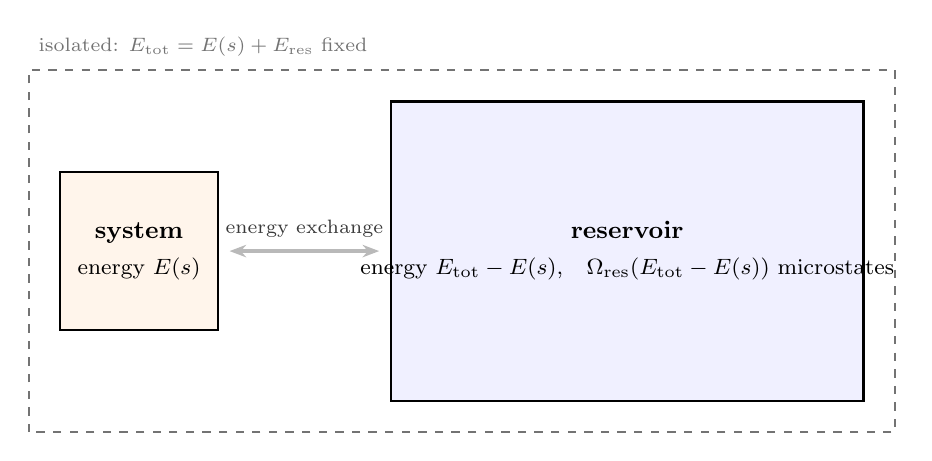
\begin{tikzpicture}[scale=1.0,transform shape]
\draw[thick,fill=orange!8] (0,0) rectangle (2.0,2.0);
\node[font=\small,align=center] at (1.0,1.0){\textbf{system}\\[2pt]\footnotesize energy $E(s)$};
\draw[thick,fill=blue!6] (4.2,-0.9) rectangle (10.2,2.9);
\node[font=\small,align=center] at (7.2,1.0){\textbf{reservoir}\\[2pt]\footnotesize energy $E_{\rm tot}-E(s)$,\quad
$\Omega_{\rm res}(E_{\rm tot}-E(s))$ microstates};
\draw[{Stealth[length=6pt]}-{Stealth[length=6pt]},very thick,gray!55] (2.15,1.0)--(4.05,1.0);
\node[font=\scriptsize,gray!45!black,anchor=south] at (3.1,1.05){energy exchange};
\draw[dashed,thick,black!55] (-0.4,-1.3) rectangle (10.6,3.3);
\node[font=\scriptsize,anchor=south west,black!55] at (-0.4,3.35){isolated: $E_{\rm tot}=E(s)+E_{\rm res}$ fixed};
\end{tikzpicture}
\caption{\SCHEM{} A small system exchanging energy with a much larger reservoir. Every microstate
of the combined (system, reservoir) pair with the same $E_{\rm tot}$ is equally likely; the
reservoir's sheer size is what turns that into an exponential law for the system alone.}
\label{fig:reservoir}
\end{figure}

Because the reservoir is enormous compared to the system, $E(s)\ll E_{\rm tot}$, so Taylor-expand
$\ln\Omega_{\rm res}$ to first order around $E_{\rm tot}$:
\begin{equation}
\ln\Omega_{\rm res}\big(E_{\rm tot}-E(s)\big)\ \approx\ \ln\Omega_{\rm res}(E_{\rm tot})\ -\
E(s)\left.\frac{d\ln\Omega_{\rm res}}{dE}\right|_{E_{\rm tot}}.
\end{equation}
Define the reservoir's entropy $S_{\rm res}=k_B\ln\Omega_{\rm res}$ (Boltzmann's entropy formula)
and \emph{define temperature thermodynamically} by $1/T=dS_{\rm res}/dE$, evaluated at the
reservoir's own energy. Substituting,
\begin{equation}
\ln\Omega_{\rm res}\big(E_{\rm tot}-E(s)\big)\ \approx\ \text{const}-\frac{E(s)}{k_BT},
\end{equation}
and exponentiating gives the \textbf{Boltzmann distribution}
\begin{equation}\label{eq:boltzmann}
p(s)\ \propto\ e^{-E(s)/k_BT}.
\end{equation}
This is derived, not assumed: it follows from nothing more than ``every accessible microstate of
an isolated system is equally likely'' plus ``the reservoir is huge.'' This manual uses the
standard lattice-model convention $k_B=1$ throughout, so temperature is measured directly in
units of energy and Eq.~\eqref{eq:boltzmann} is exactly the $p(s)\propto e^{-H(s)/T}$ asserted at
the start of \S\ref{sec:problem}.

\subsection{The partition function and free energy}
Normalising Eq.~\eqref{eq:boltzmann} requires summing over all $2^N$ microstates,
\begin{equation}\label{eq:partition}
Z=\sum_s e^{-E(s)/T},\qquad p(s)=\frac{e^{-E(s)/T}}{Z}.
\end{equation}
$Z$, the \textbf{partition function}, is the normalising constant that ``partitions'' total
probability across every microstate --- and, not coincidentally, is exactly the same
brute-force sum over $2^N$ terms that Eq.~\eqref{eq:poisson}'s cost argument shows becomes
intractable for anything but the smallest lattices. The \textbf{free energy}
\begin{equation}
F=-T\ln Z
\end{equation}
packages everything thermodynamics needs from $Z$ into one scalar, and satisfies the identity
$F=\langle E\rangle-TS$: the system's equilibrium state is the one balancing two competing
tendencies, minimising energy $\langle E\rangle$ (which favours \emph{order}) against maximising
entropy $S$ (which favours \emph{disorder}), with $T$ setting the exchange rate between them.
This is the same $F(\lambda)$ plotted schematically against the committor in
Fig.~\ref{fig:committor} --- a free-energy \emph{landscape} is just $F$ evaluated along a
coordinate $\lambda(s)$ rather than summed over all of it.

\subsection{Order, disorder, and why a phase transition exists}\label{sec:phasetransition}
At low $T$, the $TS$ term in $F=\langle E\rangle-TS$ is negligible and the system minimises
energy alone: spins align, giving the \emph{ordered} (ferromagnetic) phase. At high $T$, $TS$
dominates and the system maximises entropy instead: spins are effectively random, $m\approx0$,
the \emph{disordered} (paramagnetic) phase. In the $N\to\infty$ limit these two regimes are
separated by a sharp phase transition at $T_c$ (finite lattices smooth this into a crossover); for
the 2D ferromagnet on a square lattice this happens exactly at $T_c\approx2.269$
(\S\ref{sec:coupling}, \cite{onsager1944}).

Close to $T_c$, the competition between order and disorder produces correlated domains at every
length scale simultaneously, and single-spin-flip dynamics (Metropolis or Glauber, updating one
spin at a time) can only relax these domains locally, one flip at a time --- so the time needed
to decorrelate, $\tau_{\rm corr}$, \emph{diverges} as $T\to T_c$
(\textbf{critical slowing down}). This is measured directly, not asserted: integrated
autocorrelation time spikes to $\tau_{\rm int}=46.1$ sweeps at $T_c$ versus $1.5$--$3$ sweeps
away from criticality (\S\ref{sec:van}). This is exactly why every result in this manual is run
at $T=2.6$, comfortably above $T_c$: it keeps ``how long the chain takes to mix''
($\tau_{\rm corr}\approx1$ sweep, \S\ref{sec:tau}) cleanly separated from ``how rare is the
target event'' (set by $k$, \S\ref{sec:beyond}) --- two different kinds of difficulty this manual
is careful never to let one masquerade as the other.

%==========================================================
\section{Fundamentals: The Problem}\label{sec:problem}
%==========================================================

\subsection{A rare event, concretely}
Place $N$ magnetic moments (``spins'') on a square lattice, each pointing up or down:
$s_i\in\{-1,+1\}$. The system has energy $H(s)$, and at temperature $T$ it visits configuration
$s$ with probability $\propto e^{-H(s)/T}$ --- the Boltzmann distribution derived in
\S\ref{sec:boltzmann}. Left alone it spends essentially all its time in \emph{typical}
configurations --- call that set $A$, the \emph{bulk}: everything an equilibrium run visits
without effort.

\begin{definition}[Rare event]\label{def:rare}
Let $(s_t)_{t\ge0}$ be a Markov chain on state space $\Omega$ with stationary distribution
$\pi_s(s)\propto e^{-H(s)/T}$ (here: Glauber/Metropolis spin-flip dynamics). A \emph{rare event}
is a subset $B\subset\Omega$, disjoint from the bulk $A$, with stationary probability
$\pi:=\pi_s(B)$ small enough that i.i.d.\ sampling from $\pi_s$ needs
$M\gtrsim1/\pi$ draws (Eq.~\eqref{eq:poisson}) to observe $B$ even once at useful precision.
Rarity is therefore not an intrinsic property of $B$ --- it is a relation between $\pi$ and the
sampling budget $M$ actually available. A set with $\pi=10^{-3}$ is rare at $M=10^4$ and routine
at $M=10^8$.
\end{definition}

Concretely in this manual, $B$ is a lower tail of the energy distribution:
\begin{equation}
B=\{s: E(s)/N \le h\},
\end{equation}
with $h$ well below anything ordinary sampling produces. We want $\pi=\mathbb{P}(s\in B)$, and
$\pi$ may be $10^{-5}$ or smaller.

\subsection{Two notions of ``rare'': static tail versus dynamical hitting probability}
Definition~\ref{def:rare} is deliberately silent on \emph{how} $\pi$ is measured, and this manual
uses two different answers that must not be confused.

\textbf{Static}: $\pi_s(B)$ is a property of the equilibrium distribution alone --- a
timeless question about how much Boltzmann weight sits in $B$, answerable in principle by
direct enumeration with no dynamics at all. This is exactly what the $L=4$ exact-enumeration
gate (\S\ref{sec:validation}) computes, and it is what Eq.~\eqref{eq:poisson}'s brute-force
argument assumes it is estimating.

\textbf{Dynamical}: every $\hat\pi$ reported in a results table elsewhere in this manual
(\S\ref{sec:results}) is \emph{not} that. It is a \emph{hitting probability}: starting a
trajectory in the bulk $A$, what is the probability it reaches $B$ before returning to $A$? This
is the committor $q(s)=\mathbb{P}(\tau_B<\tau_A\mid s_0=s)$ formalized in
\S\ref{sec:corr}, and Weighted Ensemble (\S\ref{sec:we}) is built to estimate exactly this
quantity efficiently, not the static tail directly.

The two coincide under a standard metastability assumption: if dynamics mixes quickly
\emph{within} $A$ relative to the rate of leaving it toward $B$, then the long-run fraction of
time spent in $B$ (the static $\pi_s(B)$) and the per-attempt hitting probability from a
freshly-drawn bulk state (the dynamical $q$-based rate) become proportional, and both are
routinely called ``$\pi$'' without further comment --- the convention this manual follows too.
This holds throughout the $T=2.6>T_c$ regime used everywhere below, where the bulk is a single
connected basin. It is not guaranteed to hold at low temperature, where $A$ itself could
fragment into multiple metastable sub-basins separated by their own barriers --- a regime this
manual does not probe (\S\ref{sec:status}).

\subsection{The rarity ladder used throughout this manual}\label{sec:beyond}
Every empirical result below expresses rarity depth as an integer $k$ (the
\texttt{--beyond} flag), not a raw energy threshold, because a raw threshold is not portable
across lattice size, temperature, or disorder realization. Given a pilot run's population, let
$E^{\text{pilot}}_{\min}$ be the deepest energy per spin reached and $\mu$ the bulk mean energy
per spin over that same population. The target threshold is
\begin{equation}\label{eq:beyond}
h_k = E^{\text{pilot}}_{\min} - k\Delta,\qquad
\Delta=\frac{\mu-E^{\text{pilot}}_{\min}}{10},\qquad
B_k=\{s: E(s)/N \le h_k\},
\end{equation}
i.e.\ $k$ steps beyond the pilot's own most extreme observation, in units of one tenth of the
pilot's observed dynamic range. Because $h_k$ is decreasing in $k$, the family is nested,
$B_1\supset B_2\supset B_3\supset\cdots$ --- exactly the structure a multi-threshold method like
FW-CADIS (\S\ref{sec:fwcadis-theory}) is built to exploit, and the reason milestoning
(\S\ref{sec:milestoneresults}) can define ``progress'' as position within this ladder rather than a
single fixed target.

$k$ is a genuine rarity dial: \S\ref{sec:fail} measures, at fixed $L=16$, $T=2.6$, roughly one
order of magnitude drop in $\hat\pi$ per step of $k$ ($k=1$: $\hat\pi\!\approx\!2\times10^{-5}$;
$k=2$: $\hat\pi\!\approx\!10^{-6}$; $k=3$: statistics too starved to estimate reliably at
matched cost, Table~\ref{tab:reach}) --- and it is also where the ladder-difficulty discipline of
\S\ref{sec:fail} bites: too large a $k$ places $B_k$ outside what any method can resolve at
the compute available, and every comparison degrades to noise-versus-noise.

\subsection{Why brute force fails, quantitatively}
Draw $M$ independent configurations and count hits. The count is Poisson with mean $M\pi$, so
\begin{equation}\label{eq:poisson}
\frac{\sigma_{\hat\pi}}{\pi}\approx\frac{1}{\sqrt{M\pi}}.
\end{equation}
Ten percent error at $\pi=10^{-6}$ needs $M\approx10^{8}$ samples. At $L=16$ each sample costs one
sweep $=N=256$ spin updates, so that is $2.6\times10^{10}$ spin updates for one threshold.

\begin{figure}[H]\centering
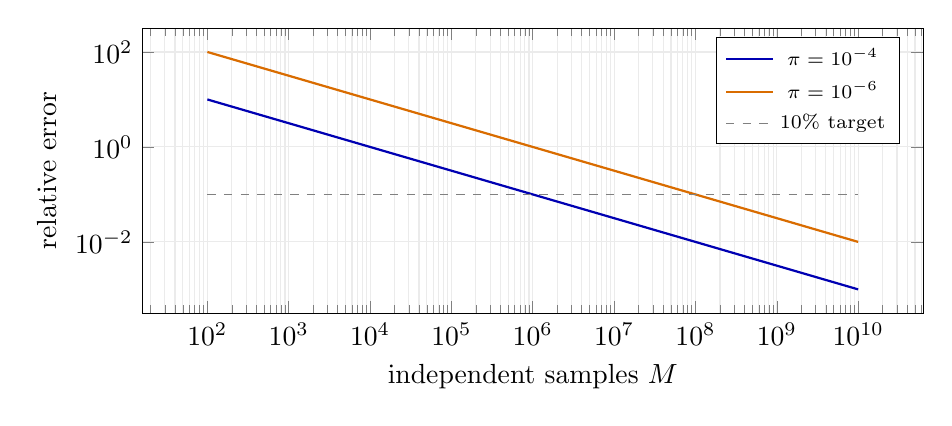
\begin{tikzpicture}
\begin{axis}[width=11.5cm,height=5.2cm,xmode=log,ymode=log,
  xlabel={independent samples $M$},ylabel={relative error},
  grid=both,grid style={gray!16},legend pos=north east,legend style={font=\scriptsize},
  every axis title/.style={font=\small}]
\addplot[thick,blue!70!black,domain=1e2:1e10,samples=40]{1/sqrt(x*1e-4)};
\addplot[thick,orange!85!black,domain=1e2:1e10,samples=40]{1/sqrt(x*1e-6)};
\addplot[dashed,gray,domain=1e2:1e10,samples=2]{0.1};
\legend{$\pi=10^{-4}$,$\pi=10^{-6}$,10\% target}
\end{axis}
\end{tikzpicture}
\caption{\SCHEM{} Exact Poisson relation \eqref{eq:poisson}, not fitted data. Each decade of
rarity costs a decade of samples. This is the wall the project exists to get around.}
\end{figure}

\subsection{The idea behind every solution}
All enhanced-sampling methods make the same move: \textbf{spend effort where it matters}. If we
knew, for each configuration $s$, the probability that a trajectory from $s$ reaches $B$ before
returning to the bulk $A$, we could steer computation toward promising configurations. That
probability is the committor $q(s)$. The rest of this manual is about why $q$ is the optimal guide,
why transport theory already has it under another name, and how to approximate it.

%==========================================================
\section{The Lattice and the Model}\label{sec:lattice}
%==========================================================

\subsection{Geometry and Hamiltonian}
On an $L\times L$ lattice with periodic boundaries, $N=L^2$,
\begin{equation}
H(s)=-\sum_{\langle i,j\rangle}J_{ij}s_is_j,\qquad E(s)/N = H(s)/N,
\end{equation}
with $\langle i,j\rangle$ over nearest-neighbour pairs and periodic wrapping
$s_{(x+L)\bmod L,\,y}=s_{x,y}$, $s_{x,\,(y+L)\bmod L}=s_{x,y}$.

\begin{figure}[H]\centering
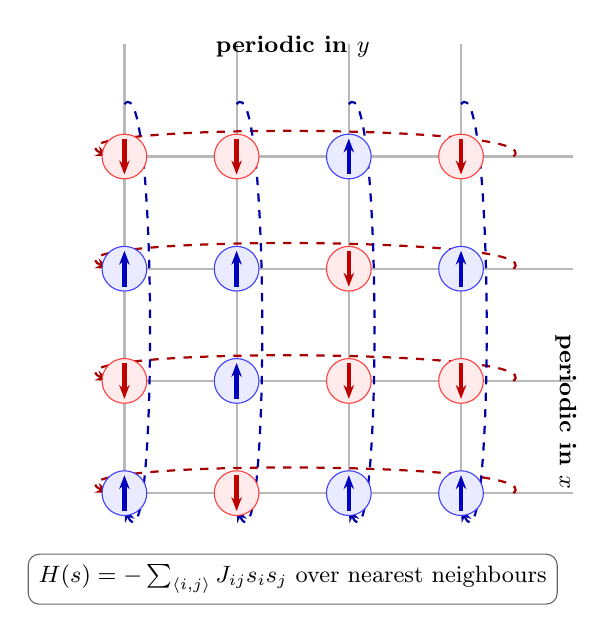
\begin{tikzpicture}[scale=0.95,transform shape]
\foreach \x in {0,1.5,3,4.5}{\foreach \y in {0,1.5,3,4.5}{
  \draw[thick,gray!55] (\x,\y)--(\x+1.5,\y);
  \draw[thick,gray!55] (\x,\y)--(\x,\y+1.5);}}
\foreach \x in {0,1.5,3,4.5}{\draw[thick,gray!55] (\x,4.5)--(\x,5.2);}
\foreach \y in {0,1.5,3,4.5}{\draw[thick,gray!55] (4.5,\y)--(5.2,\y);}
\foreach \y in {0,1.5,3,4.5}{\pgfmathsetmacro{\yp}{\y+0.45}
  \draw[red!65!black,dashed,thick,-{Stealth[length=5pt]}] (5.2,\y) .. controls (5.75,\yp) and (-1.25,\yp) .. (-0.2,\y);}
\foreach \x in {0,1.5,3,4.5}{\pgfmathsetmacro{\xp}{\x+0.45}
  \draw[blue!65!black,dashed,thick,-{Stealth[length=5pt]}] (\x,5.2) .. controls (\xp,5.75) and (\xp,-1.25) .. (\x,-0.2);}
\def\spins{{1,-1,1,1,-1,1,-1,-1,1,1,-1,1,-1,-1,1,-1}}
\foreach \x [count=\xi from 0] in {0,1.5,3,4.5}{
 \foreach \y [count=\yi from 0] in {0,1.5,3,4.5}{
  \pgfmathsetmacro{\idx}{int(\yi*4+\xi)}\pgfmathsetmacro{\s}{int(\spins[\idx])}
  \ifnum\s=1
   \node[circle,draw=blue!75,fill=blue!8,inner sep=2pt,minimum size=17pt] at (\x,\y){};
   \draw[-{Stealth[length=5pt]},ultra thick,blue!75!black] (\x,\y-0.24)--(\x,\y+0.24);
  \else
   \node[circle,draw=red!75,fill=red!8,inner sep=2pt,minimum size=17pt] at (\x,\y){};
   \draw[-{Stealth[length=5pt]},ultra thick,red!75!black] (\x,\y+0.24)--(\x,\y-0.24);
  \fi}}
\node[anchor=south,font=\small] at (2.25,5.7){\textbf{periodic in $y$}};
\node[anchor=west,rotate=-90,font=\small] at (5.9,2.25){\textbf{periodic in $x$}};
\node[draw=black!60,fill=white,rounded corners,inner sep=4pt,font=\small] at (2.25,-1.15)
 {$H(s)=-\sum_{\langle i,j\rangle}J_{ij}s_is_j$ over nearest neighbours};
\end{tikzpicture}
\caption{\SCHEM{} The $L\times L$ lattice, drawn at $L=4$. Blue $=$ spin up, red $=$ spin down,
solid lines are coupling bonds $J_{ij}$, dashed arrows are the periodic identifications.}
\label{fig:lattice}
\end{figure}

\subsection{Two coupling choices}\label{sec:coupling}
\begin{itemize}[leftmargin=*]
\item \textbf{Ferromagnet}: $J_{ij}=+1$ uniformly. Ordering transition at
$\beta_c=\tfrac12\ln(1+\sqrt2)\approx0.4407$, i.e. $T_c\approx2.269$. Magnetisation $m$ is an
obviously informative reaction coordinate.
\item \textbf{Edwards--Anderson spin glass}: $J_{ij}$ drawn independently and \textbf{bimodally},
$J_{ij}\in\{-1,+1\}$ with equal probability, quenched by a fixed seed. Low-energy states are
disordered, $m\approx0$ regardless of energy, and a hand-picked coordinate is expected to fail.
\end{itemize}
All results use $T=2.6$ (above $T_c$), $L=16$ for full scale, $L=4$ for exact-enumeration gates.

\begin{warnbox}{Correction to earlier drafts}
An earlier version of this manual stated $J_{ij}\sim\mathcal{N}(0,\sigma_J^2)$. The reference
implementation uses \texttt{rng.choice([-1.0, 1.0])} --- the $\pm J$ bimodal model. The two differ
in ground-state degeneracy and universality class, so the distinction is not cosmetic.
\end{warnbox}

\subsection{Frustration: why this landscape is hard}\label{sec:frustration}
A plaquette is \emph{frustrated} when the product of its four bonds is negative: no spin
assignment satisfies all four simultaneously.

\begin{figure}[H]\centering
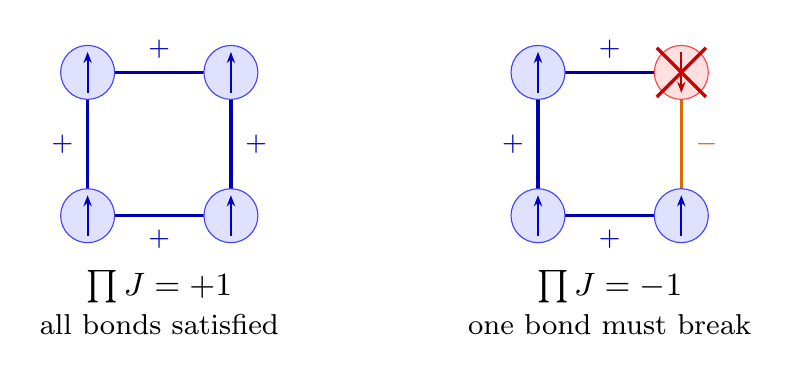
\begin{tikzpicture}[scale=1.3,transform shape]
\begin{scope}
\draw[very thick,blue!70!black] (0,0)--(1.4,0) node[midway,below,font=\scriptsize]{$+$};
\draw[very thick,blue!70!black] (0,1.4)--(1.4,1.4) node[midway,above,font=\scriptsize]{$+$};
\draw[very thick,blue!70!black] (0,0)--(0,1.4) node[midway,left,font=\scriptsize]{$+$};
\draw[very thick,blue!70!black] (1.4,0)--(1.4,1.4) node[midway,right,font=\scriptsize]{$+$};
\foreach \x/\y in {0/0, 1.4/0, 0/1.4, 1.4/1.4}{
  \node[circle,draw=blue!75,fill=blue!12,minimum size=15pt,inner sep=0pt] at (\x,\y) {};
  \draw[-{Stealth[length=4pt]},thick,blue!75!black] (\x,\y-0.2)--(\x,\y+0.2);}
\node[font=\small,align=center] at (0.7,-0.85){$\prod J=+1$\\ \footnotesize all bonds satisfied};
\end{scope}
\begin{scope}[xshift=4.4cm]
\draw[very thick,blue!70!black] (0,0)--(1.4,0) node[midway,below,font=\scriptsize]{$+$};
\draw[very thick,blue!70!black] (0,1.4)--(1.4,1.4) node[midway,above,font=\scriptsize]{$+$};
\draw[very thick,blue!70!black] (0,0)--(0,1.4) node[midway,left,font=\scriptsize]{$+$};
\draw[very thick,orange!85!black] (1.4,0)--(1.4,1.4) node[midway,right,font=\scriptsize]{$-$};
\foreach \x/\y in {0/0, 1.4/0, 0/1.4}{
  \node[circle,draw=blue!75,fill=blue!12,minimum size=15pt,inner sep=0pt] at (\x,\y) {};
  \draw[-{Stealth[length=4pt]},thick,blue!75!black] (\x,\y-0.2)--(\x,\y+0.2);}
\node[circle,draw=red!75,fill=red!12,minimum size=15pt,inner sep=0pt] at (1.4,1.4){};
\draw[-{Stealth[length=4pt]},thick,red!75!black] (1.4,1.6)--(1.4,1.2);
\draw[red!80!black,line width=1.2pt] (1.16,1.16)--(1.64,1.64);
\draw[red!80!black,line width=1.2pt] (1.16,1.64)--(1.64,1.16);
\node[font=\small,align=center] at (0.7,-0.85){$\prod J=-1$\\ \footnotesize one bond must break};
\end{scope}
\end{tikzpicture}
\caption{\SCHEM{} Left: all four bonds ferromagnetic, product $+1$, a satisfying assignment
exists. Right: one antiferromagnetic bond makes the product $-1$; whichever spins are chosen, at
least one bond is unsatisfied. Frustration is what makes the energy landscape rugged.}
\label{fig:frustration}
\end{figure}

For the disorder sample used throughout ($L=16$, seed 0), direct measurement gives:
\begin{center}\small
\begin{tabular}{lc}\toprule
antiferromagnetic bonds ($J=-1$) & 233 of 512\\
frustrated plaquettes & \textbf{126 of 256 (49.2\%)}\\
\bottomrule\end{tabular}
\end{center}
Nearly half the lattice cannot be locally satisfied. There is no growing domain and no visible
order parameter --- which is why magnetisation carries little information here, and why a
\emph{learned} coordinate is worth the effort.

\subsection{From two dimensions to three: what would change}\label{sec:threed}
Everything above is stated for the 2D square lattice this manual actually runs. None of it was
tried in 3D. This subsection makes precise what would have to change and, more usefully, what
would not --- because the two lists are not the same size.

\textbf{Geometry.} A simple-cubic lattice replaces the square one: $N=L^3$ sites, each with $6$
nearest neighbours (coordination number $z=6$) instead of $4$, periodic wrapping in all three
directions. The Hamiltonian keeps the identical form,
$H(s)=-\sum_{\langle i,j\rangle}J_{ij}s_is_j$, summed over the now-larger bond set. Nothing about
the physics setup of \S\ref{sec:lattice}--\S\ref{sec:coupling} needs rethinking, only re-indexing.

\begin{figure}[H]\centering
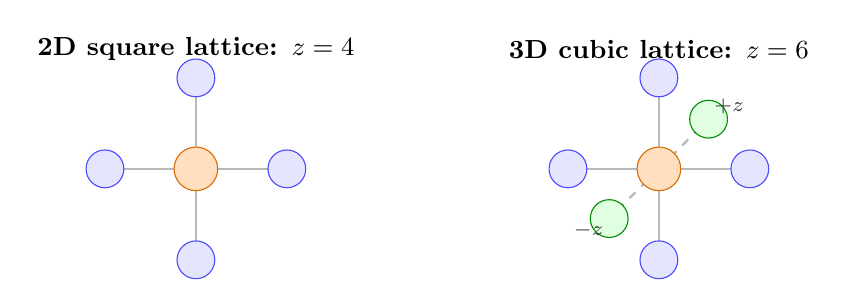
\begin{tikzpicture}[scale=1.05,transform shape]
\node[font=\small\bfseries] at (1.0,2.75){2D square lattice: $z=4$};
\draw[thick,gray!55] (1.0,1.3)--(2.1,1.3);
\draw[thick,gray!55] (1.0,1.3)--(-0.1,1.3);
\draw[thick,gray!55] (1.0,1.3)--(1.0,2.4);
\draw[thick,gray!55] (1.0,1.3)--(1.0,0.2);
\node[circle,draw=blue!70,fill=blue!10,minimum size=13pt,inner sep=0pt] at (2.1,1.3){};
\node[circle,draw=blue!70,fill=blue!10,minimum size=13pt,inner sep=0pt] at (-0.1,1.3){};
\node[circle,draw=blue!70,fill=blue!10,minimum size=13pt,inner sep=0pt] at (1.0,2.4){};
\node[circle,draw=blue!70,fill=blue!10,minimum size=13pt,inner sep=0pt] at (1.0,0.2){};
\node[circle,draw=orange!85!black,fill=orange!25,minimum size=15pt,inner sep=0pt] at (1.0,1.3){};
\begin{scope}[xshift=5.6cm]
\node[font=\small\bfseries] at (1.0,2.75){3D cubic lattice: $z=6$};
\draw[thick,gray!55] (1.0,1.3)--(2.1,1.3);
\draw[thick,gray!55] (1.0,1.3)--(-0.1,1.3);
\draw[thick,gray!55] (1.0,1.3)--(1.0,2.4);
\draw[thick,gray!55] (1.0,1.3)--(1.0,0.2);
\draw[thick,gray!55,dashed] (1.0,1.3)--(1.601,1.901);
\draw[thick,gray!55,dashed] (1.0,1.3)--(0.399,0.699);
\node[circle,draw=blue!70,fill=blue!10,minimum size=13pt,inner sep=0pt] at (2.1,1.3){};
\node[circle,draw=blue!70,fill=blue!10,minimum size=13pt,inner sep=0pt] at (-0.1,1.3){};
\node[circle,draw=blue!70,fill=blue!10,minimum size=13pt,inner sep=0pt] at (1.0,2.4){};
\node[circle,draw=blue!70,fill=blue!10,minimum size=13pt,inner sep=0pt] at (1.0,0.2){};
\node[circle,draw=green!55!black,fill=green!12,minimum size=13pt,inner sep=0pt] at (1.601,1.901){};
\node[circle,draw=green!55!black,fill=green!12,minimum size=13pt,inner sep=0pt] at (0.399,0.699){};
\node[font=\scriptsize,gray!45!black] at (1.85,2.05){$+z$};
\node[font=\scriptsize,gray!45!black] at (0.15,0.55){$-z$};
\node[circle,draw=orange!85!black,fill=orange!25,minimum size=15pt,inner sep=0pt] at (1.0,1.3){};
\end{scope}
\end{tikzpicture}
\caption{\SCHEM{} Nearest-neighbour coordination: a 2D square lattice (left) gives each spin
$z=4$ neighbours (blue); a 3D cubic lattice (right) adds a third axis (green, dashed bonds shown
foreshortened for depth), giving $z=6$. The Hamiltonian's form,
$H(s)=-\sum_{\langle i,j\rangle}J_{ij}s_is_j$, is unchanged --- only the bond count per site
(orange, centre) grows.}
\label{fig:coordination}
\end{figure}

\textbf{The exact reference disappears.} The 2D square-lattice ferromagnet has Onsager's exact
solution, $T_c\approx2.269$ \cite{onsager1944} --- the number this manual's own $T=2.6$ choice is
pinned against (\S\ref{sec:phasetransition}). No exact solution exists for the 3D cubic Ising
model; $T_c$ is known only from high-precision numerics, currently
$T_c/J\approx4.5115$ (from $K_c=J/k_BT_c=0.2216544(3)$) via large-scale cluster Monte Carlo
\cite{talapov1996}. Any 3D extension of this manual would inherit a numerical, not exact,
temperature scale to calibrate against.

\textbf{The $L=4$ exact-enumeration gate breaks, and this is the serious obstacle.} Every
validation claim in this manual (\S\ref{sec:validation} and throughout) rests on checking $L=4$
against direct enumeration of all $2^N$ microstates. In 2D, $L=4$ means $N=16$ and $2^{16}=65536$
--- trivial. In 3D, $L=4$ means $N=64$ and $2^{64}\approx1.8\times10^{19}$ --- utterly
infeasible. Keeping exact enumeration tractable in 3D means dropping to roughly $L=2$
($N=8$, $2^8=256$), a lattice almost certainly too small to exercise the WE/committor machinery
the way $L=4$ does in 2D (too few bins, too little structure). This is not a matter of more
compute; it is the validation \emph{strategy itself} that does not survive the dimension change,
and any 3D extension would need a different anchor (series expansions, or a published high-$L$
numerical benchmark, in place of exact enumeration).

\begin{figure}[H]\centering
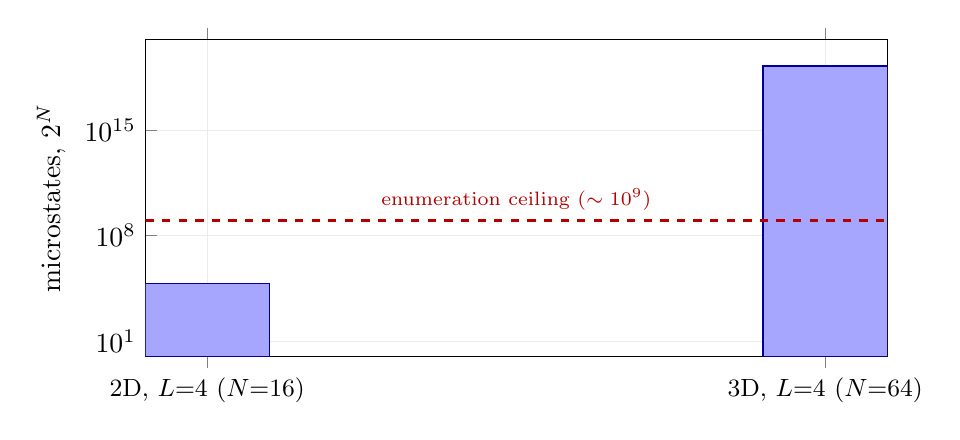
\begin{tikzpicture}
\begin{axis}[width=11cm,height=5.6cm,ybar,bar width=45pt,ymode=log,
symbolic x coords={2D,3D},xtick=data,
xticklabels={{2D, $L{=}4$ ($N{=}16$)},{3D, $L{=}4$ ($N{=}64$)}},
x tick label style={font=\small,align=center},
ylabel={microstates, $2^N$},
ymin=1,ymax=1e21,
grid=major,grid style={gray!16}]
\addplot[fill=blue!35,draw=blue!60!black] coordinates {(2D,65536) (3D,1.8e19)};
\draw[dashed,red!70!black,thick] (rel axis cs:0,0.4286) -- (rel axis cs:1,0.4286)
node[midway,above,font=\scriptsize,red!70!black]{enumeration ceiling ($\sim10^9$)};
\end{axis}
\end{tikzpicture}
\caption{\SCHEM{} Exact-enumeration cost at $L=4$: trivial in 2D ($2^{16}=65536$ states),
utterly infeasible in 3D ($2^{64}\approx1.8\times10^{19}$ states) --- fourteen orders of
magnitude beyond any practical enumeration budget. This is why the $L=4$ validation strategy
used throughout this manual (\S\ref{sec:validation}) cannot simply be re-run one dimension
higher.}
\label{fig:statespace}
\end{figure}

\textbf{The spin-glass physics changes qualitatively, not just quantitatively.} The 2D
Edwards--Anderson spin glass used throughout this manual has \emph{no finite-temperature
ordering transition} --- it orders, if at all, only as $T\to0$ \cite{binderyoung1986}. Every run
in this manual, however cold, is therefore formally still in a single (extremely rough) phase:
frustration produces a rugged landscape without a genuine thermodynamic phase boundary to cross.
The 3D $\pm J$ Edwards--Anderson model is different in kind: it has a genuine finite-temperature
spin-glass transition, $T_g/J\approx1.10$ (from $\beta_c=0.908(2)$) \cite{hasenbusch2008}. A 3D
extension could therefore ask the rare-event question on either side of a real phase boundary ---
a qualitatively different and arguably richer problem than anything tested here, not merely a
bigger version of it.

\textbf{Sampling cost scales faster with $L$.} One Monte Carlo sweep costs $N$ spin updates
(\S\ref{sec:problem}), and $N=L^3$ grows faster than the 2D $N=L^2$ used everywhere in this
manual's cost estimates. Matching the $N=256$ scale used throughout (2D, $L=16$) needs only
$L\approx6$ in 3D ($L=6\Rightarrow N=216$); running 3D at the same $L=16$ used everywhere here
instead means $N=4096$, a $16\times$ larger per-sweep cost, and correspondingly larger WE
populations at fixed bin occupancy. This changes the achievable-scale calculus quantitatively
even before asking whether the harder physics helps or hurts variance reduction.

\textbf{What would \emph{not} need to change.} This is the encouraging half. The rare-event
sampling machinery this manual is actually about --- the committor identity
(\S\ref{sec:corr}), Weighted Ensemble split/merge (\S\ref{sec:we}), milestoning labels
(\S\ref{sec:objectives}), and FW-CADIS allocation (\S\ref{sec:fwcadis-theory}) --- operates
entirely on the energy/committor coordinate and the Markov transition kernel, neither of which
knows or cares whether the underlying lattice is 2D or 3D. Only lattice generation, neighbour-list
construction, and the VAN's autoregressive raster order (\S\ref{sec:van}) would need to change;
none of \S\ref{sec:we}--\S\ref{sec:learned} would need modification in principle.

\textbf{Concretely: how the rare event would be sought.} The recipe is identical to
\S\ref{sec:problem}--\S\ref{sec:learned}, re-run on the cubic lattice. A pilot run at the chosen
$T$ (comfortably above the relevant $T_c$ or $T_g$, \S\ref{sec:phasetransition}) gives
$E^{\rm pilot}_{\min}$ and $\mu$; the rarity ladder $B_k$ of Eq.~\eqref{eq:beyond} is defined from
those two numbers exactly as before --- the formula is written entirely in terms of pilot-run
statistics, so it \emph{re-calibrates itself} to whatever energy landscape the cubic lattice
produces, with no change to the formula, only to which lattice generates the pilot. Weighted
Ensemble bins along the same coordinate choices (energy $E$, or a trained $I_\theta(s)$) using the
identical split/merge rule (\S\ref{sec:we}); milestoning labels (\S\ref{sec:objectives}) place
intermediate targets along the same ladder. The one piece that does change shape is $I_\theta$'s
input: a network trained on a 2D $L\times L$ raster must instead consume an $L\times L\times L$
voxel grid (or its flattened $N=L^3$ vector) --- a change to the network's input geometry, not to
what it is trained to predict or how WE uses its output.

\textbf{Concretely: removing critical slowing down in 3D.} The VAN strategy of \S\ref{sec:van}
sidesteps critical slowing down entirely because it never runs local-update dynamics: it draws
whole configurations one variable at a time from a learned autoregressive factorisation
$p_\theta(s)=\prod_i q_\theta(s_i\mid s_{<i})$, so every sample is independent by construction
regardless of how close $T$ is to $T_c$. That argument never references dimensionality, so it
carries over to 3D unchanged in substance: the raster scan over the $L\times L$ grid
(Fig.~\ref{fig:van}) becomes a scan over the $L\times L\times L$ volume --- concretely, sweep
through $L$ two-dimensional layers in sequence, raster-scanning each layer before moving to the
next, so ``earlier in the scan'' still means ``earlier'' in one consistent global order --- and
the 2D masked convolutions (PixelCNN-style) generalise directly to 3D masked (``causal'')
convolutions, an established technique for autoregressive models over volumetric data. Nothing
about the variational training objective changes. Critical slowing down itself is not a 2D
peculiarity: local-update dynamics relax collective modes near \emph{any} continuous transition,
2D or 3D, and recent five-loop field-theoretic estimates of the dynamic critical exponent for
Model~A (single-spin-flip) dynamics give $z\approx2.14(2)$ in 2D against $z\approx2.0235(8)$ in 3D
\cite{adzhemyan2022} --- both close to the diffusive value $z\approx2$, so the VAN's advantage
over local updates is not expected to be dramatically larger or smaller in 3D than the
$\tau_{\rm int}=46.1$-sweep spike already measured at $T_c$ in 2D (\S\ref{sec:van}); it removes
the same qualitative bottleneck for the same reason.

This project did not run 3D (\S\ref{sec:status} lists it as an untouched push-to-scale
direction); this subsection exists to state precisely where the real obstacles are --- the broken
exact-enumeration gate above all --- not to claim the extension has been tried.

%==========================================================
\section{The Transport--Statistical Mechanics Correspondence}\label{sec:corr}
%==========================================================

\subsection{Two fields, one function}
In radiation shielding one asks: given a source and a detector behind a thick shield, what
fraction of particles reach the detector? Almost none do --- the same rare-event structure.
Transport theory answers with the \emph{adjoint flux} $\psi^\dagger$, defined by
$H^\dagger\psi^\dagger=\sigma_d$ with a source placed \emph{at the detector}. Its physical
reading: $\psi^\dagger(P)$ is the expected contribution to the tally of one particle introduced
at phase-space point $P$ --- its \emph{importance}.

In spin dynamics the committor is
\begin{equation}
q(s)=\mathbb{P}(\tau_B<\tau_A\mid s_0=s),\qquad \tau_X=\min\{t\ge0: s_t\in X\},
\end{equation}
satisfying the discrete backward Kolmogorov equation on intermediate states
$\Ical=\Omega\setminus(A\cup B)$,
\begin{equation}\label{eq:bke}
\sum_{s'}K(s\to s')\,q(s')=q(s)\quad\forall s\in\Ical,\qquad q|_A=0,\ q|_B=1.
\end{equation}

\begin{figure}[H]\centering
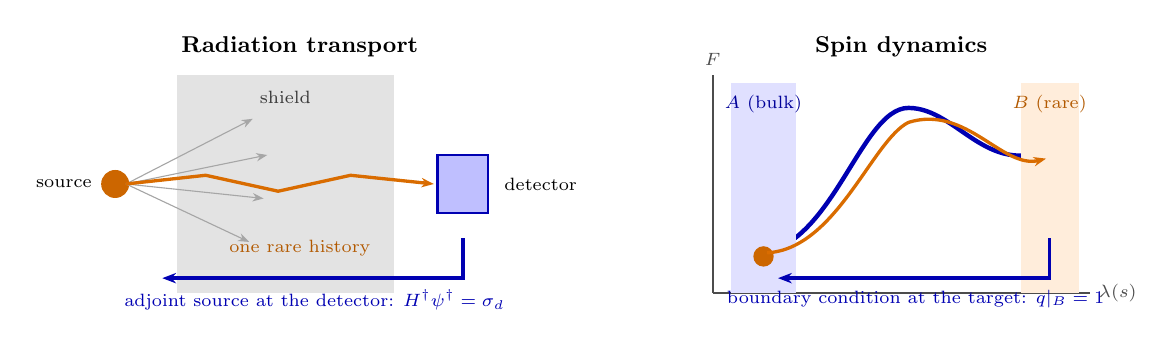
\begin{tikzpicture}[scale=0.92,transform shape]
% ---------- transport panel
\begin{scope}
\fill[gray!22] (1.2,0) rectangle (4.2,3.0);
\node[font=\scriptsize,gray!45!black] at (2.7,2.7){shield};
\node[circle,fill=orange!80!black,minimum size=11pt,inner sep=0pt] (src) at (0.35,1.5){};
\node[font=\scriptsize,anchor=east] at (0.15,1.5){source};
\draw[fill=blue!25,draw=blue!70!black,thick] (4.8,1.1) rectangle (5.5,1.9);
\node[font=\scriptsize,anchor=west] at (5.6,1.5){detector};
\foreach \a/\o in {0.9/0.35,0.4/0.55,-0.2/0.5,-0.8/0.3}{
 \draw[-{Stealth[length=4pt]},gray!70] (0.5,1.5)--(1.9+\o,1.5+\a);}
\draw[-{Stealth[length=4.5pt]},very thick,orange!85!black] (0.5,1.5)--(1.6,1.62)--(2.6,1.4)--(3.6,1.62)--(4.75,1.5);
\node[font=\scriptsize,orange!70!black] at (2.9,0.62){one rare history};
\draw[-{Stealth[length=5pt]},very thick,blue!70!black] (5.15,0.75)--(5.15,0.20)--(1.0,0.20);
\node[font=\scriptsize,blue!70!black,anchor=north] at (3.1,0.16){adjoint source at the detector: $H^\dagger\psi^\dagger=\sigma_d$};
\node[font=\small\bfseries] at (2.9,3.4){Radiation transport};
\end{scope}
% ---------- spin panel
\begin{scope}[xshift=8.6cm]
\draw[thick,black!70] (0,0)--(0,3.0) node[above,font=\scriptsize]{$F$};
\draw[thick,black!70] (0,0)--(5.2,0) node[right,font=\scriptsize]{$\lambda(s)$};
\draw[ultra thick,blue!70!black] (0.4,0.55) .. controls (1.6,0.35) and (2.0,2.55) .. (2.7,2.55)
 .. controls (3.4,2.55) and (3.8,1.5) .. (4.8,2.05);
\fill[blue!12] (0.25,0) rectangle (1.15,2.9);
\fill[orange!14] (4.25,0) rectangle (5.05,2.9);
\node[font=\scriptsize,blue!60!black] at (0.7,2.6){$A$ (bulk)};
\node[font=\scriptsize,orange!70!black] at (4.65,2.6){$B$ (rare)};
\node[circle,fill=orange!80!black,minimum size=8pt,inner sep=0pt] at (0.7,0.5){};
\draw[-{Stealth[length=4.5pt]},very thick,orange!85!black]
 (0.75,0.55) .. controls (1.7,0.6) and (2.2,2.1) .. (2.7,2.35) .. controls (3.5,2.6) and (4.0,1.7) .. (4.6,1.85);
\draw[-{Stealth[length=5pt]},very thick,blue!70!black] (4.65,0.75)--(4.65,0.20)--(0.9,0.20);
\node[font=\scriptsize,blue!70!black,anchor=north] at (2.8,0.16){boundary condition at the target: $q|_B=1$};
\node[font=\small\bfseries] at (2.6,3.4){Spin dynamics};
\end{scope}
\end{tikzpicture}
\caption{\SCHEM{} The same structure twice. Both quantities are defined \emph{backward from the
target}: the adjoint source sits at the detector, the committor boundary condition sits on the
rare set. That shared direction is the whole correspondence, and it is why transport's
variance-reduction toolkit transfers.}
\label{fig:corr}
\end{figure}

\begin{table}[H]\centering\small
\caption{Correspondence used throughout this work.}
\begin{tabular}{p{3.0cm}p{6.0cm}p{6.0cm}}\toprule
& \textbf{Radiation transport} & \textbf{Spin dynamics}\\\midrule
Phase-space point & $(r,\Omega,E)$ & microstate $s\in\{-1,+1\}^N$\\
Forward operator & Boltzmann $H$ & Markov kernel $K$\\
Target & detector response $R$ & hitting probability of $B$\\
Importance & adjoint flux $\psi^\dagger$ & committor $q(s)$\\
Optimal biasing & adjoint-weighted tilt & Doob $h$-transform $\widetilde K$\\
Weight control & weight windows & weighted ensemble (WE)\\
Global objective & FW-CADIS & uniform relative error across thresholds\\
Efficiency metric & $\mathrm{FOM}=1/(\sigma^2_{\mathrm{rel}}T)$ & identical\\\midrule
Physical origin of $K$ & real scattering/absorption, cross-sections & thermal spin-flip
acceptance (Metropolis/Glauber)\\
State space & continuous, discretized (groups, ordinates) & already finite, $2^N$, exact\\
Natural biasing coordinate & position/direction/energy (geometric) & \textbf{none} --- must be
learned\\
\bottomrule\end{tabular}
\end{table}

\subsection{How exact is this correspondence, really?}
The claim above is easy to overstate. Three things are true at once, and this manual is careful
to keep them separate.

\textbf{The linear-algebra core is an exact identity, not an analogy.} Real transport
calculations never solve the continuous operator equation $H^\dagger\psi^\dagger=\sigma_d$
directly: phase space is first discretized into energy groups and a finite set of directions
(\emph{multigroup, discrete-ordinates} transport), turning it into a finite linear system
$(\mathbb I-\mathbf K)\boldsymbol\psi^\dagger=\boldsymbol\sigma_d$ for some transition operator
$\mathbf K$ packaging streaming and scattering between cells. That is term-for-term the same
linear system as Eq.~\eqref{eq:bke}: a (sub)stochastic operator $K$, a source/boundary term, one
solve. Nothing about $K$'s physical origin enters the algebra --- the identity holds for
\emph{any} Markov process with an absorbing target set, which is exactly why it transfers to
spin dynamics with zero modification to the mathematics.

\textbf{The physical mechanism generating $K$ has nothing in common.} Transport's $K$ encodes a
real particle's free flight interrupted by real scattering and absorption events, with rates set
by cross-sections measured in a lab. Spin dynamics' $K$ encodes the acceptance probability of a
proposed single-spin flip under a thermal bath at temperature $T$. There is no mean free path, no
cross-section, and no particle in the spin problem --- a ``walker'' here is a bookkeeping device
for one member of a population of independent simulation replicas, not a physical object. The
correspondence is a shared \emph{mathematical} structure, not a shared physical mechanism, and
conflating the two would overclaim what has actually been unified.

\textbf{Spin systems are strictly easier for this correspondence, in one specific sense.}
Multigroup or discrete-ordinates transport pays a discretization error that must be separately
verified, usually against measurement, since the exact continuous answer is rarely available at
all. A spin lattice's state space is already finite and discrete --- $2^N$ configurations, no
truncation, no group structure to choose. That is exactly why $L=4$ can be checked against exact
enumeration to within $\sim2\%$ (\S\ref{sec:validation}): there is no discretization step to
introduce error, only sampling error. In that narrow sense, the spin lattice is a \emph{cleaner}
testbed for this correspondence than the shielding problem that motivated it.

\textbf{Spin systems are strictly harder in the one place it matters most.} Transport's
importance function is biased and binned along a natural, low-dimensional, physically meaningful
coordinate --- position, direction, energy --- chosen from the geometry of the shield, not
learned. Spin configurations have no such coordinate: there is no ``distance to the detector''
for a $256$-spin configuration. Energy and magnetization are the closest analogues, and
\S\ref{sec:frustration} shows the obvious one (magnetization) fails outright on the spin glass.
This absence, not anything about the linear algebra, is the actual reason
\S\ref{sec:learned} needs a \emph{learned} importance coordinate $I_\theta(s)$ at all --- the
single largest way this problem instance diverges from the shielding problem it borrows its
toolkit from.

\subsection{Why the committor is optimal}
\begin{theorem}[Zero-variance sampling]\label{thm:zv}
Let $q$ solve \eqref{eq:bke} and define the tilted kernel
$\widetilde K(s\to s')=K(s\to s')\,q(s')/q(s)$ on $\Ical$. Then every trajectory reaching $B$
carries the same importance weight and the estimator variance vanishes.
\end{theorem}
\begin{proof}
$\widetilde K$ is stochastic: $\sum_{s'}\widetilde K(s\to s')=q(s)^{-1}\sum_{s'}K(s\to s')q(s')=1$
by \eqref{eq:bke}. For a path $\gamma=(s_0,\dots,s_K)$ with $s_K\in B$, the density ratio
telescopes,
\begin{equation}
\frac{\widetilde{\mathcal{P}}(\gamma)}{\mathcal{P}(\gamma)}
=\prod_{t=0}^{K-1}\frac{q(s_{t+1})}{q(s_t)}=\frac{q(s_K)}{q(s_0)}=\frac{1}{q(s_0)},
\end{equation}
using $q(s_K)=1$. Hence $w(\gamma)=q(s_0)$, a constant, so $\mathrm{Var}[w]=0$.
\end{proof}

\begin{okbox}{Verified numerically}
On a solvable 1D absorbing walk on $\{0,\dots,15\}$ with $\pi=1.14\times10^{-3}$, tilting by the
exact committor gave measured relative variance $\sim10^{-30}$ --- zero to machine precision.
Crucially, tilting by an \emph{approximate} committor \emph{without} weight windows was
\textbf{worse than plain naive Monte Carlo}. That fragility is why every learned-coordinate
result in this project uses weighted ensemble rather than raw importance reweighting.
\end{okbox}

\subsection{Free energy versus committor}
Theorem~\ref{thm:zv} is an existence statement, not an algorithm: computing $q$ exactly needs a
linear system of size $2^N$. Its practical content is a \emph{target} for approximation.

\begin{figure}[H]\centering
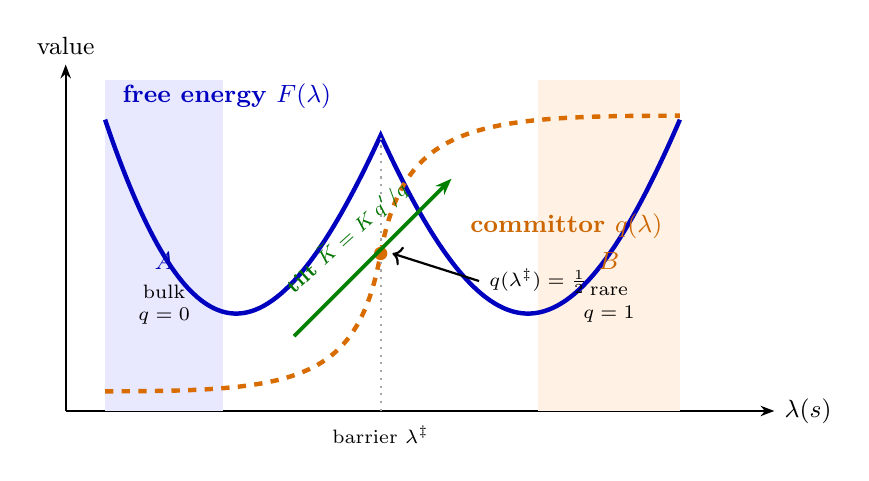
\begin{tikzpicture}[scale=1.0,transform shape]
\draw[-{Stealth[length=5pt]},thick] (0,0)--(9.0,0) node[right,font=\small]{$\lambda(s)$};
\draw[-{Stealth[length=5pt]},thick] (0,0)--(0,4.4) node[above,font=\small]{value};
\fill[blue!9] (0.5,0) rectangle (2.0,4.2);
\fill[orange!11] (6.0,0) rectangle (7.8,4.2);
\draw[ultra thick,blue!75!black] (0.5,3.7) .. controls (1.6,0.45) and (2.6,0.45) .. (4.0,3.5)
 .. controls (5.4,0.45) and (6.4,0.45) .. (7.8,3.7);
\node[blue!75!black,font=\small\bfseries,anchor=west] at (0.6,4.0){free energy $F(\lambda)$};
\draw[ultra thick,orange!85!black,dashed] (0.5,0.25) .. controls (2.9,0.25) and (3.7,0.35) .. (4.0,2.0)
 .. controls (4.3,3.65) and (5.2,3.75) .. (7.8,3.75);
\node[orange!80!black,font=\small\bfseries,anchor=east] at (7.7,2.35){committor $q(\lambda)$};
\node[font=\small\bfseries,blue!70!black] at (1.25,1.9){$A$};
\node[font=\scriptsize,align=center] at (1.25,1.35){bulk\\$q=0$};
\node[font=\small\bfseries,orange!80!black] at (6.9,1.9){$B$};
\node[font=\scriptsize,align=center] at (6.9,1.35){rare\\$q=1$};
\draw[dotted,thick,gray!70] (4.0,0)--(4.0,3.5);
\node[anchor=north,font=\scriptsize] at (4.0,-0.06){barrier $\lambda^\ddagger$};
\node[circle,fill=orange!85!black,inner sep=1.7pt] at (4.0,2.0){};
\draw[<-,thick] (4.15,2.0)--(5.25,1.65) node[right,font=\scriptsize]{$q(\lambda^\ddagger)=\tfrac12$};
\draw[-{Stealth[length=6pt]},line width=1.3pt,green!50!black] (2.9,0.95)--(4.9,2.95);
\node[green!45!black,font=\scriptsize,rotate=42,anchor=south] at (3.75,2.0)
 {\textbf{tilt} $\widetilde K=K\,q'/q$};
\end{tikzpicture}
\caption{\SCHEM{} The committor is smooth and monotone where the free energy has a barrier. Tilting
by $q$ converts the barrier into a downhill drift, which is why the estimator becomes
variance-free. Curves are illustrative shapes, not measured profiles.}
\label{fig:committor}
\end{figure}

%==========================================================
\section{Weighted Ensemble: Mechanics}\label{sec:we}
%==========================================================

\subsection{The algorithm}
WE is the statistical-mechanics name for split/Russian-roulette weight windows. A population of
weighted walkers is propagated under \emph{unbiased} dynamics, binned along a progress
coordinate, and each occupied bin is resampled to a fixed occupancy $N_0$ with its total weight
conserved.

\begin{figure}[H]\centering
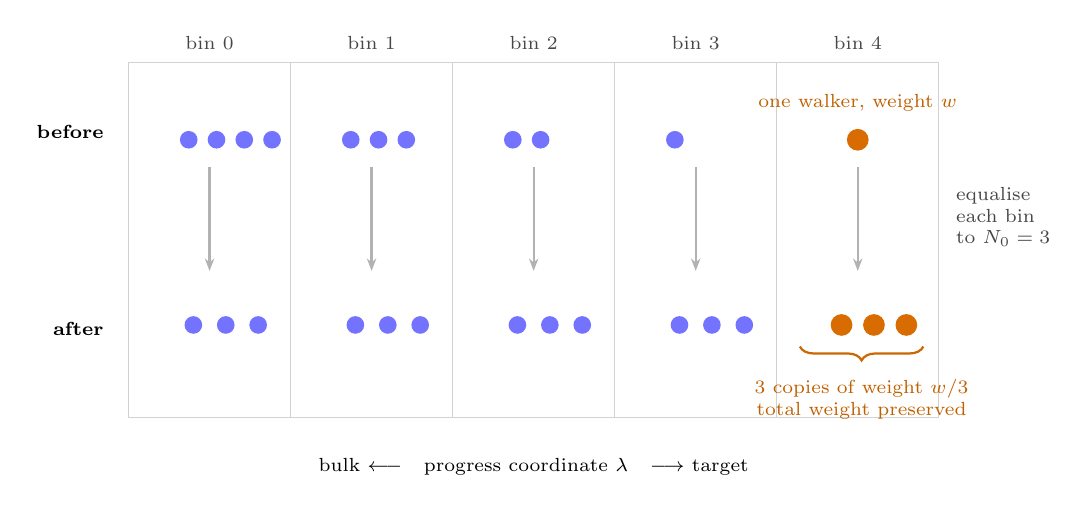
\begin{tikzpicture}[scale=0.98,transform shape]
\foreach \i in {0,1,2,3,4}{
 \draw[gray!35] (\i*2.1,0) rectangle (\i*2.1+2.1,4.6);
 \node[font=\scriptsize,gray!55!black] at (\i*2.1+1.05,4.85){bin \i};}
\node[font=\scriptsize,anchor=east,align=right] at (-0.2,3.7){\textbf{before}};
\node[font=\scriptsize,anchor=east,align=right] at (-0.2,1.15){\textbf{after}};
\node[font=\scriptsize,anchor=north] at (5.25,-0.4){bulk $\longleftarrow$\quad progress coordinate $\lambda$\quad $\longrightarrow$ target};
\foreach \i/\n in {0/4,1/3,2/2,3/1}{
 \foreach \k in {1,...,\n}{
  \node[circle,fill=blue!55,minimum size=6.5pt,inner sep=0pt] at (\i*2.1+0.42+0.36*\k,3.6){};}}
\node[circle,fill=orange!85!black,minimum size=8pt,inner sep=0pt] at (4*2.1+1.05,3.6){};
\node[font=\scriptsize,orange!75!black,anchor=south] at (4*2.1+1.05,3.85){one walker, weight $w$};
\foreach \i in {0,1,2,3,4}{
 \draw[-{Stealth[length=4.5pt]},thick,gray!60] (\i*2.1+1.05,3.25)--(\i*2.1+1.05,1.9);}
\node[font=\scriptsize,gray!55!black,anchor=west,align=left] at (10.6,2.6){equalise\\each bin\\to $N_0=3$};
\foreach \i in {0,1,2,3}{\foreach \k in {1,2,3}{
  \node[circle,fill=blue!55,minimum size=6.5pt,inner sep=0pt] at (\i*2.1+0.42+0.42*\k,1.2){};}}
\foreach \k in {1,2,3}{
  \node[circle,fill=orange!85!black,minimum size=8pt,inner sep=0pt] at (4*2.1+0.42+0.42*\k,1.2){};}
\draw[decorate,decoration={brace,amplitude=5pt,mirror},orange!80!black,thick]
  (4*2.1+0.3,0.92)--(4*2.1+1.9,0.92);
\node[font=\scriptsize,orange!75!black,anchor=north,align=center] at (4*2.1+1.1,0.62){3 copies of weight $w/3$\\ total weight preserved};
\end{tikzpicture}
\caption{\SCHEM{} The whole method in one picture. A lone walker that fluctuates into a deep bin
is \emph{split} into $N_0$ copies which then explore from there; crowded bulk bins are merged
back down. Weight bookkeeping keeps the estimator exactly unbiased, so \emph{any} binning
coordinate is safe --- a poor one costs efficiency, never correctness.}
\label{fig:we}
\end{figure}

\begin{theorem}[Unbiasedness]
Splitting walker $(s_i,w_i)$ into $K$ copies of weight $w_i/K$ contributes
$\sum_k (w_i/K)\,O(s_i)=w_i O(s_i)$. Merging $(s_1,w_1),(s_2,w_2)$ into one survivor of weight
$w_1+w_2$ chosen with probability $w_j/(w_1+w_2)$ has expectation $w_1O(s_1)+w_2O(s_2)$.
Both are identities, so bin weights --- and therefore the estimator --- are preserved exactly.
\end{theorem}

\subsection{Validation against exact enumeration}\label{sec:validation}
At $L=4$ the state space is enumerable and WE reproduces the exact $P(m)$ to a mean
$|\Delta\ln P|$ of $0.006$--$0.024$ across three tested regimes. At $L=20$, WE reaches roughly two
decades deeper into the magnetisation tail than naive Monte Carlo at matched cost: naive's floor
is $|m|=0.886$ ($P\approx6\times10^{-6}$), where it returns zero samples and hence zero
information, while WE reaches $|m|=0.932$ ($P\approx2.4\times10^{-7}$).

%==========================================================
\section{Failure Modes, Diagnosed}\label{sec:fail}
%==========================================================

Three implementation faults each produced plausible-looking wrong numbers. Each is documented
with the measurement that exposed it, because the diagnostic reasoning is the reusable part.

\subsection{Failure 1: the resampling interval}\label{sec:tau}
Splitting only helps if the copies stay correlated long enough to be split \emph{again} before
they relax. The system's own correlation time is therefore a hard constraint on $\tau$.

\begin{figure}[H]\centering
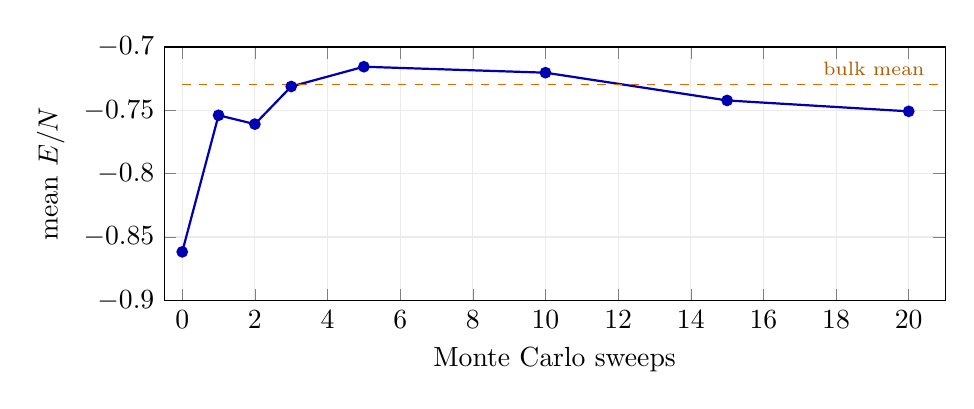
\begin{tikzpicture}
\begin{axis}[width=11.5cm,height=4.8cm,xlabel={Monte Carlo sweeps},ylabel={mean $E/N$},
 grid=both,grid style={gray!16},ymin=-0.90,ymax=-0.70,xmin=-0.5,xmax=21]
\addplot[thick,blue!70!black,mark=*,mark size=1.7]
 coordinates {(0,-0.8617) (1,-0.7539) (2,-0.7609) (3,-0.7312) (5,-0.7156) (10,-0.7203) (15,-0.7422) (20,-0.7508)};
\addplot[dashed,orange!85!black,domain=0:21,samples=2]{-0.7299};
\node[font=\scriptsize,orange!70!black,anchor=south east] at (axis cs:20.7,-0.7299){bulk mean};
\end{axis}
\end{tikzpicture}
\caption{\MEAS{} Starting from the 20 deepest configurations of an equilibrated population, the
mean energy returns to the bulk value within \textbf{one sweep}. Hence
$\tau_{\mathrm{corr}}\approx1$ sweep at $T=2.6$.}
\label{fig:relax}
\end{figure}

With $\tau=20$, every split copy is an independent equilibrium sample by the next resampling. WE
then degenerates into naive sampling with bookkeeping overhead.

\begin{figure}[H]\centering
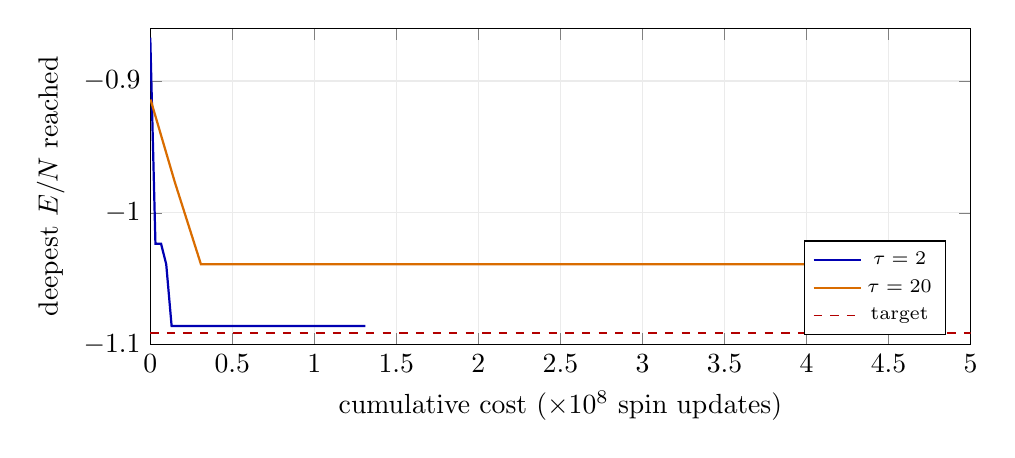
\begin{tikzpicture}
\begin{axis}[width=12cm,height=5.6cm,
 xlabel={cumulative cost ($\times10^8$ spin updates)},ylabel={deepest $E/N$ reached},
 grid=both,grid style={gray!16},xmin=0,xmax=5,ymin=-1.10,ymax=-0.86,
 legend pos=south east,legend style={font=\scriptsize}]
\addplot[thick,blue!70!black] coordinates {(0.0002,-0.8672) (0.0317,-1.0234) (0.0659,-1.0234) (0.0975,-1.0391) (0.1303,-1.0859) (0.1638,-1.0859) (0.1968,-1.0859) (0.2288,-1.0859) (0.2607,-1.0859) (0.2937,-1.0859) (0.3269,-1.0859) (0.3592,-1.0859) (0.3928,-1.0859) (0.4262,-1.0859) (0.4581,-1.0859) (0.4911,-1.0859) (0.5247,-1.0859) (0.5579,-1.0859) (0.5896,-1.0859) (0.6228,-1.0859) (0.6558,-1.0859) (0.6883,-1.0859) (0.7207,-1.0859) (0.7535,-1.0859) (0.7860,-1.0859) (0.8192,-1.0859) (0.8518,-1.0859) (0.8854,-1.0859) (0.9189,-1.0859) (0.9517,-1.0859) (0.9845,-1.0859) (1.0177,-1.0859) (1.0506,-1.0859) (1.0832,-1.0859) (1.1172,-1.0859) (1.1508,-1.0859) (1.1844,-1.0859) (1.2155,-1.0859) (1.2474,-1.0859) (1.2804,-1.0859) (1.3113,-1.0859)};
\addplot[thick,orange!85!black] coordinates {(0.0020,-0.9141) (0.1495,-0.9766) (0.3092,-1.0391) (0.4649,-1.0391) (0.6287,-1.0391) (0.7946,-1.0391) (0.9605,-1.0391) (1.1244,-1.0391) (1.2780,-1.0391) (1.4418,-1.0391) (1.5974,-1.0391) (1.7572,-1.0391) (1.9272,-1.0391) (2.0890,-1.0391) (2.2569,-1.0391) (2.4146,-1.0391) (2.5723,-1.0391) (2.7341,-1.0391) (2.8938,-1.0391) (3.0618,-1.0391) (3.2256,-1.0391) (3.3874,-1.0391) (3.5471,-1.0391) (3.7069,-1.0391) (3.8666,-1.0391) (4.0264,-1.0391) (4.1902,-1.0391) (4.3418,-1.0391) (4.5036,-1.0391) (4.6633,-1.0391) (4.7923,-1.0391)};
\addplot[dashed,red!70!black,domain=0:5,samples=2]{-1.0912};
\legend{$\tau=2$,$\tau=20$,target}
\end{axis}
\end{tikzpicture}
\caption{\MEAS{} Identical bins, one seed. At $\tau=2$ the front reaches $-1.086$ by cost
$1.3\times10^8$ and plateaus \emph{because it has arrived}. At $\tau=20$ it plateaus at $-1.039$
\emph{because it is stuck}, then spends $3.7\times$ more budget going nowhere. Both plateaus look
alike; only one is convergence.}
\label{fig:front}
\end{figure}

\begin{table}[H]\centering\small
\caption{\MEAS{} Front penetration versus $\tau$ at matched cost. Bin 0 is the target bin.}
\begin{tabular}{ccccc}\toprule
$\tau$ & iterations & deepest bin & iterations with a target hit & cost\\\midrule
20 & 150 & 8 & 0/150 & $4.8\times10^8$\\
4 & 400 & 2 & 0/400 & $2.6\times10^8$\\
1 & 800 & \textbf{0} & \textbf{2/800} & $1.4\times10^8$\\
\bottomrule\end{tabular}
\end{table}

\begin{warnbox}{Correction to earlier drafts}
Earlier text stated that changing $\tau=20\to4$ ``restored correlation control''. The table shows
$\tau=4$ still fails to reach the target bin at this depth. With $\tau_{\mathrm{corr}}\approx1$,
$\tau=4$ is a partial mitigation; $\tau\in\{1,2\}$ is required at deep targets. Results quoted at
$\tau=4$ should state the depth at which they were taken --- at shallow targets $\tau=4$ may well
suffice.
\end{warnbox}

\subsection{Failure 2: bin-ladder placement}
Bins must span $[\,\text{target}\to\text{bulk}\,]$ \emph{from the first iteration}. If the range
is seeded adaptively from random initial configurations, its upper edge sits near $E/N\approx0$
while equilibrium sits near $-0.73$, so over half the ladder covers states never visited. Fixing
the range to $(h-4/N,\ \mu+2\sigma)$ from a pilot run removes this.

\begin{table}[H]\centering\small
\caption{\MEAS{} Controlled test: only the upper edge changed, same seeds.}
\begin{tabular}{lccc}\toprule
upper edge & bin width & target hits / 300 iters & cost\\\midrule
$-0.5689$ ($\mu+2\sigma$) & $0.01076$ & 0,\ 1 & $1.6\times10^8$\\
$-0.7300$ (bulk mean) & $0.00754$ & 0,\ 1 & $9.8\times10^7$\\
\bottomrule\end{tabular}
\end{table}

The tighter edge costs 40\% less for the same penetration. Note it does \emph{not} change the hit
rate: bin width affects cost, not reach. An earlier diagnosis attributed reach to bin width; the
controlled test above refutes that and it is reported as such.

\subsection{Failure 3: an unreachable target}
Recall the rarity ladder $h_k=E^{\text{pilot}}_{\min}-k\Delta$ of Eq.~\eqref{eq:beyond}
(\S\ref{sec:beyond}). Sweeping $k$:

\begin{table}[H]\centering\small
\caption{\MEAS{} Target reachability, $\tau=2$, 300 iterations, two independent seeds.}
\label{tab:reach}
\begin{tabular}{cccc}\toprule
$k$ (\texttt{--beyond}) & threshold $h$ & hits / 300 & $\hat\pi$ (seed 0, seed 1)\\\midrule
1 & $-1.0356$ & 10,\ 9 & $2.00\times10^{-5}$,\ $1.93\times10^{-5}$\\
2 & $-1.0634$ & 1,\ 3 & $0$,\ $2.13\times10^{-6}$\\
3 & $-1.0912$ & 0,\ 1 & $0$,\ $1.01\times10^{-7}$\\
\bottomrule\end{tabular}
\end{table}

At $k=1$ two independent seeds agree to 4\%: converged. At $k=3$ the estimate is a coin flip. The
WE front asymptotes near $E/N\approx-1.09$, so $k=3$ places the target \emph{at the edge of
reachability} and every method returns starved statistics.

\begin{okbox}{Ladder-difficulty discipline}
Comparing methods where the baseline itself fails to observe the event compares noise to noise.
Every comparison in \S\ref{sec:results} is reported at a depth where the reference methods reach
0, or nearly 0, zero-replicas --- found by backing off from a harder target until this holds.
\end{okbox}

%==========================================================
\section{The Learned Importance Coordinate}\label{sec:learned}
%==========================================================

\subsection{Why a network, and why it is safe to try}
The committor is a function on $2^{256}$ states and cannot be tabulated. But it need not be
exact: WE stays unbiased for \emph{any} binning coordinate, so a poor $I_\theta$ costs efficiency,
never correctness. The failure mode is a slow run, not a wrong answer.

\subsection{Removing critical slowing down: the VAN}\label{sec:van}
Generating decorrelated reference configurations is a separate difficulty from rare-event
sampling, and it is handled separately. A variational autoregressive network samples
configurations directly by factorising in raster-scan order,
\begin{equation}
q_\theta(s)=\prod_{i=1}^{N}q_\theta(s_i\mid s_{<i}),
\end{equation}
with causal masking so site $i$ depends only on previously generated sites.

\begin{figure}[H]\centering
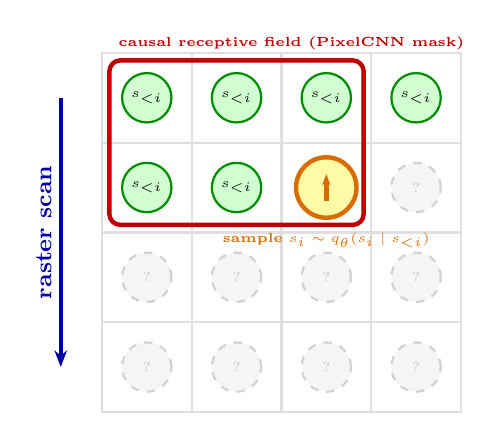
\begin{tikzpicture}[scale=0.95,transform shape]
\foreach \x in {0,1.2,2.4,3.6}{\foreach \y in {0,1.2,2.4,3.6}{
  \draw[gray!25,thick] (\x,\y) rectangle (\x+1.2,\y+1.2);}}
\foreach \p in {(0.6,4.2),(1.8,4.2),(3.0,4.2),(4.2,4.2),(0.6,3.0),(1.8,3.0)}{
  \draw[fill=green!18,draw=green!55!black,thick] \p circle (0.33);
  \node[font=\tiny] at \p {$s_{<i}$};}
\node[circle,draw=orange!85!black,fill=yellow!35,ultra thick,minimum size=23pt,inner sep=0pt] at (3.0,3.0){};
\draw[-{Stealth[length=4pt]},ultra thick,orange!85!black] (3.0,2.82)--(3.0,3.18);
\node[anchor=north,orange!85!black,font=\tiny] at (3.0,2.52){\textbf{sample} $s_i\sim q_\theta(s_i\mid s_{<i})$};
\foreach \p in {(4.2,3.0),(0.6,1.8),(1.8,1.8),(3.0,1.8),(4.2,1.8),(0.6,0.6),(1.8,0.6),(3.0,0.6),(4.2,0.6)}{
  \draw[fill=gray!8,draw=gray!35,dashed,thick] \p circle (0.33);
  \node[gray!45,font=\tiny] at \p {?};}
\draw[red!75!black,ultra thick,rounded corners] (0.1,2.5) rectangle (3.5,4.7);
\node[red!75!black,anchor=south west,font=\tiny] at (0.1,4.72){\textbf{causal receptive field (PixelCNN mask)}};
\draw[-{Stealth[length=6pt]},line width=1.3pt,blue!65!black] (-0.55,4.2)--(-0.55,0.6);
\node[blue!65!black,rotate=90,anchor=south,font=\small] at (-0.55,2.4){\textbf{raster scan}};
\end{tikzpicture}
\caption{\SCHEM{} Autoregressive generation. Type-A masking (first layer) zeroes the centre pixel
to prevent self-dependence; type-B masking (later layers) retains it.}
\label{fig:van}
\end{figure}

\begin{okbox}{Measured}
At $L=32$ the integrated autocorrelation time of ordinary Metropolis sampling spikes to
$\tau_{\mathrm{int}}=46.1$ sweeps at $T_c\approx2.269$, versus 1.5--3 sweeps away from
criticality. The VAN samples independently by construction and pays none of this. This is a
\emph{speed} result, orthogonal to the rare-event problem.
\end{okbox}

\subsection{Training objectives}\label{sec:objectives}
\begin{itemize}[leftmargin=*]
\item \textbf{Surrogate rollout label.} Binary committor labels collapse to all-zero for a
genuinely rare target, so the network regresses the best progress value reached in $K$ short
rollouts --- a dense, monotone surrogate.
\item \textbf{Milestoning.} Intermediate thresholds are placed along the ladder from bulk to
target; a configuration's label estimates progress toward the \emph{next} milestone rather than
the final target. Closer to the theoretical object while avoiding label collapse.
\item \textbf{Self-consistency (Kim \& Cai).} Label-free: minimise violation of
$\sum_j K(s\to j)I(j)=I(s)$ with $I=1$ on the target.
\end{itemize}

\subsection{Label orientation}
Training targets must satisfy \textbf{larger value $=$ closer to the target}. With milestones
$m_0$ (bulk) $\dots$ $m_{M-1}$ (target), the correct continuous label is
\begin{equation}
\ell(s)=\mathrm{clip}\!\left(\frac{E_{\text{best}}(s)-m_0}{m_{M-1}-m_0},0,1\right).
\end{equation}

\begin{warnbox}{Latent bug: inverted labels --- caught, no reported number affected}
An implementation assigned labels via \texttt{np.searchsorted(np.sort(milestones), E\_best)}.
Because the target is the \emph{most negative} milestone, ascending sort places it at index 0: a
walker reaching the target received label $0.0$ and one staying in the bulk received $0.857$. The
network was trained as an \textbf{anti}-importance function, $\ell_{\text{wrong}}=1-\ell$.

\textbf{Why the WE results survive.} The inversion is an \emph{affine} map, and
\texttt{we\_estimate} bins by \texttt{linspace(c.min(), c.max())} then \texttt{digitize},
resampling every occupied bin to the same occupancy. No directional term appears anywhere in
that loop, so an affine flip permutes bin \emph{labels} while leaving the induced
\emph{partition} of walkers identical (verified directly: 26 occupied bins, same grouping under
$c$ and $1-c$). WE binning is orientation-agnostic, so \S\ref{sec:results} stands.

\textbf{Where it would have been fatal.} Any \emph{directional} use of $I_\theta$: Doob tilting
$\widetilde K=K\,I(j)/I(i)$, source biasing $\hat q\propto\psi^\dagger q$, or depth-keyed
FW-CADIS allocation. An inverted $I$ drives walkers \emph{away} from the target --- precisely the
failure the 1D toy walk showed is worse than naive. Fixed before any such use.
\end{warnbox}

\subsection{Is $I_\theta$ informative, or a noisy copy of energy?}
A nested-regression diagnostic settles this. Fit the rare-event label on $E$ alone, on $I_\theta$
alone, and on both:

\begin{table}[H]\centering\small
\caption{\MEAS{} Incremental-$R^2$ diagnostic, EA spin glass, $L=16$, matched training budget
(MSE $1.0\to0.271$ over 20 epochs).}
\begin{tabular}{lc}\toprule
quantity & value\\\midrule
Pearson $\mathrm{corr}(I_\theta,E/N)$ & $-0.614$\\
fraction of $\mathrm{Var}(I_\theta)$ unexplained by $E/N$ & $0.623$\\
$R^2$ (label $\sim E/N$) & $0.358$\\
$R^2$ (label $\sim I_\theta$) & $0.577$\\
$R^2$ (label $\sim E/N+I_\theta$) & $0.608$\\
\textbf{incremental $R^2$ from $I_\theta$} & $\mathbf{+0.250}$\\
\bottomrule\end{tabular}
\end{table}

$+0.250$ is far above the diagnostic's own noise threshold ($0.02$): $I_\theta$ carries
substantial genuine information about the spin glass that energy does not.

\begin{warnbox}{Retracted sub-result}
A first attempt at this diagnostic used an undertrained network and was retracted. An
undertrained network's output is uncorrelated with \emph{everything}, including energy, which is
not evidence of new information --- it is evidence of noise.
\end{warnbox}

\subsection{FW-CADIS as a loss-weighting principle}\label{sec:fwcadis-theory}
Bin occupancy is uneven --- the bulk dominates --- so an unweighted MSE is fit almost entirely to
near-bulk configurations. FW-CADIS weights the adjoint source by the forward flux so every region
attains comparable relative error rather than optimising one detector. Transplanted:
\begin{equation}
\mathcal{L}_{\mathrm{FW}}=\sum_{b=1}^{M}\frac{1}{n_b}\sum_{i\in\text{bin }b}
\big(I_\theta(s_i)-\ell(s_i)\big)^2,
\end{equation}
with $n_b$ the occupancy of bin $b$: inverse-frequency weighting, the discrete analogue of
forward-flux normalisation.

%==========================================================
\section{Results}\label{sec:results}
%==========================================================

\subsection{Milestoning: a clean regime for comparison, but wildly seed-dependent}\label{sec:milestoneresults}
On the EA spin glass at $L=16$, one threshold step beyond the pilot extreme, every method reaches
$0/10$ zero-replicas --- the cleanest regime obtained in this project by the usual
ladder-difficulty standard. The first run in this regime gave WE[$I_\theta$] a 14\% FOM win over
WE[$E$]; that result did \emph{not} reproduce (\S\ref{man:seedbug}) and the honest picture, after
sweeping seventeen independent network initializations, is a small, seed-noisy effect that cannot
yet be distinguished from zero.

\begin{table}[H]\centering\small
\caption{\MEAS{} EA spin glass, $L=16$, $T=2.6$, \texttt{beyond}$=1$, 10 replicas, milestoning
labels, seventeen independent training runs of the identical configuration. naive, WE[$m$], and
WE[$E$] are bit-identical across all runs (deterministic; WE[$E$] does not depend on the trained
network). Seed 0 was run twice independently and reproduced bit-for-bit, confirming the seeding
fix of \S\ref{man:seedbug} is complete.}
\begin{tabular}{lcccc}\toprule
Method & $\hat\pi$ & rel. s.d. & FOM & zero-replicas\\\midrule
naive & $5.29\times10^{-5}$ & 0.225 & $\mathbf{1.48\times10^{-7}}$ & 0/10\\
WE[$m$] & $5.55\times10^{-5}$ & 0.201 & $1.17\times10^{-7}$ & 0/10\\
WE[$E$] & $4.49\times10^{-5}$ & 0.209 & $4.22\times10^{-8}$ & 0/10\\
WE[$I_\theta$], unseeded run 1 & $5.03\times10^{-5}$ & 0.174 & $4.81\times10^{-8}$ ($+14\%$) & 0/10\\
WE[$I_\theta$], unseeded run 2 & $4.52\times10^{-5}$ & 0.204 & $3.48\times10^{-8}$ ($-17\%$) & 0/10\\
WE[$I_\theta$], seeds 0--15 & \multicolumn{4}{l}{range $2.29$--$8.94\times10^{-8}$ ($-52\%$ to $+112\%$), all 0/10}\\
\bottomrule\end{tabular}
\end{table}

\begin{figure}[H]\centering
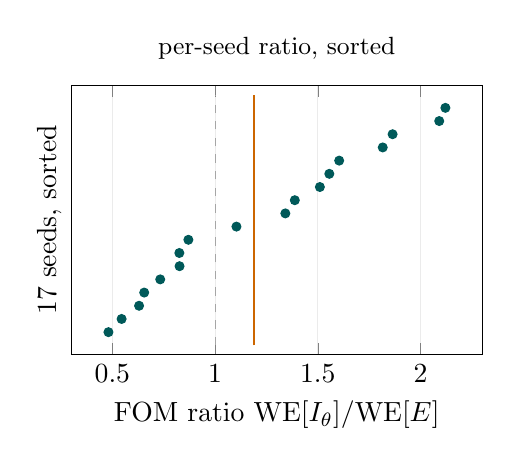
\begin{tikzpicture}
\begin{axis}[width=6.8cm,height=5.0cm,xlabel={FOM ratio WE[$I_\theta$]/WE[$E$]},
 ylabel={17 seeds, sorted},ytick=\empty,xmin=0.3,xmax=2.3,grid=major,grid style={gray!16},
 title={\small per-seed ratio, sorted}]
\addplot[only marks,mark=*,mark size=1.6pt,color=teal!70!black] coordinates
 {(0.481,0) (0.545,1) (0.630,2) (0.655,3) (0.733,4) (0.827,5) (0.826,6) (0.870,7)
  (1.104,8) (1.342,9) (1.388,10) (1.510,11) (1.556,12) (1.604,13) (1.816,14)
  (1.864,15) (2.091,16) (2.121,17)};
\draw[dashed,gray!70] (axis cs:1,-1) -- (axis cs:1,18) node[above,font=\tiny]{no effect};
\draw[thick,orange!80!black] (axis cs:1.19,-1) -- (axis cs:1.19,18);
\end{axis}
\end{tikzpicture}\hfill
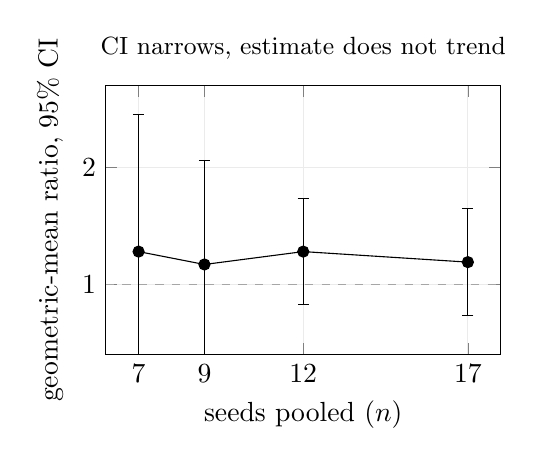
\begin{tikzpicture}
\begin{axis}[width=6.6cm,height=5.0cm,xlabel={seeds pooled ($n$)},
 ylabel={geometric-mean ratio, 95\% CI},xtick={7,9,12,17},ymin=0.4,ymax=2.7,
 grid=major,grid style={gray!16},title={\small CI narrows, estimate does not trend}]
\addplot[color=black,mark=*,error bars/.cd,y dir=both,y explicit] coordinates
 {(7,1.28) +- (0,1.17) (9,1.17) +- (0,0.89) (12,1.28) +- (0,0.45) (17,1.19) +- (0,0.455)};
\draw[dashed,gray!70] (axis cs:6,1) -- (axis cs:18,1);
\end{axis}
\end{tikzpicture}
\caption{\MEAS{} Left: all seventeen per-seed FOM ratios (sorted); orange line marks the pooled
two-level-bootstrap median. Right: the four tracked checkpoints as seeds were added --- the point
estimate bounces between $1.17\times$ and $1.28\times$ while the CI width shrinks monotonically
($1.73\to1.36\to1.18\to0.91$), the signature of averaging down noise around a small,
sign-unresolved effect, not a shrinking or growing true one.}
\label{fig:manseedsweep}
\end{figure}

Pooling all seventeen seeds with a two-level bootstrap (outer resample over seeds, inner resample
over each seed's 10 replicas) gives a geometric-mean FOM ratio of $1.19\times$, 95\% CI
$[0.84,\,1.75]$ --- includes 1, i.e.\ \textbf{not statistically significant even at 17 independent
seeds}. Extrapolating the observed CI-width-vs-$n$ scaling ($1/\sqrt n$, confirmed to match
observation), excluding 1 would need roughly 100 total seeds ($\sim$40h more compute); not
pursued further given the already-thorough characterization. \textbf{Naive Monte Carlo still has
the best raw FOM at this rarity in every seed} --- variance reduction has not yet earned back its
overhead here, the same lesson the 1D toy walk showed in miniature.

A candidate explanation --- that WE[$I_\theta$]'s adaptive (rather than fixed) bin range was the
driver of the seed variance --- was tested and ruled out: an empirically calibrated fixed range,
run head-to-head against the adaptive baseline on matched net-seeds, made both the mean ratio and
the rel.\ s.d.\ \emph{worse}, not better. The variance is intrinsic to what each trained network
learns, not an artifact of how its output is binned.

\subsection{Pushing deeper fails, and bin count is ruled out as the fix}
At one step rarer, WE[$I_\theta$] scores below WE[$E$] in every configuration tried: default bins
at two replica counts, and a $1.8\times$ larger bin count. Raising $n_{\text{bins}}$ from 50 to 90
made WE[$I_\theta$] \emph{worse} ($8.36\times10^{-9}\to5.36\times10^{-9}$), which rules out bin
resolution as the explanation --- a genuine resolution shortfall would improve with more bins.
The mechanism is structural: the learned coordinate's walker-population cost scales with bin
count, whereas a discretised coordinate like energy saturates a small fixed number of bins.

\subsection{Self-consistency objective: a result that did not survive scrutiny}
\begin{table}[H]\centering\small
\caption{\MEAS{} Bootstrapped FOM ratios, $L=16$, shallowest calibrated target. Ratio $>1$ favours
the self-consistency objective.}
\begin{tabular}{lcccc}\toprule
Comparison & $R$ & median ratio & 95\% CI & significant?\\\midrule
self-consistent / surrogate & 10 & 1.83 & $[0.49,\ 9.23]$ & no\\
self-consistent / surrogate & 30 & 1.39 & $[0.65,\ 2.95]$ & no\\
self-consistent / WE[$E$] & 10 & 1.19 & $[0.33,\ 4.95]$ & no\\
self-consistent / WE[$E$] & 30 & 1.07 & $[0.55,\ 2.09]$ & no\\
\bottomrule\end{tabular}
\end{table}

Tripling the replica count tightened both intervals \emph{and} moved both medians toward 1. The
point estimate itself receded as evidence accumulated --- the signature of noise, not signal. The
initially exciting ``$+87\%$'' became a statistically insignificant $+39\%$ with an interval
including no difference at all.

\subsection{FW-CADIS: real cost advantage, no flattening}
The implementation gates clean against exact enumeration at $L=4$ (ratios within $\sim2\%$ of
exact for every threshold, both allocations, both models). At scale, the flattening the method is
named for does not appear.

\begin{figure}[H]\centering
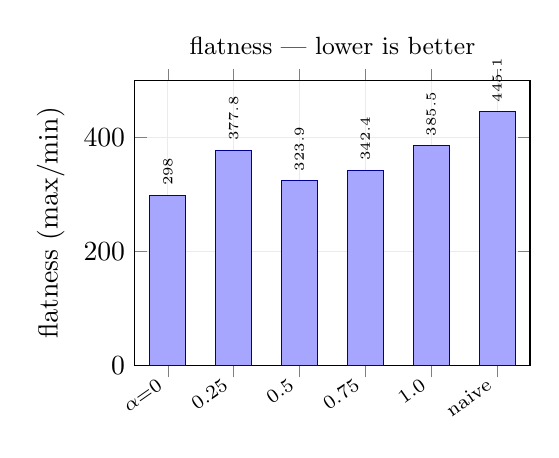
\begin{tikzpicture}
\begin{axis}[width=6.6cm,height=5.2cm,ybar,bar width=13pt,
 symbolic x coords={$\alpha$=0,0.25,0.5,0.75,1.0,naive},xtick=data,
 x tick label style={font=\scriptsize,rotate=35,anchor=east},
 ylabel={flatness (max/min)},ymin=0,ymax=500,
 title={\small flatness --- lower is better},grid=major,grid style={gray!16},
 nodes near coords,every node near coord/.append style={font=\tiny,rotate=90,anchor=west}]
\addplot[fill=blue!35,draw=blue!60!black] coordinates
 {($\alpha$=0,298.0) (0.25,377.8) (0.5,323.9) (0.75,342.4) (1.0,385.5) (naive,445.1)};
\end{axis}
\end{tikzpicture}\hfill
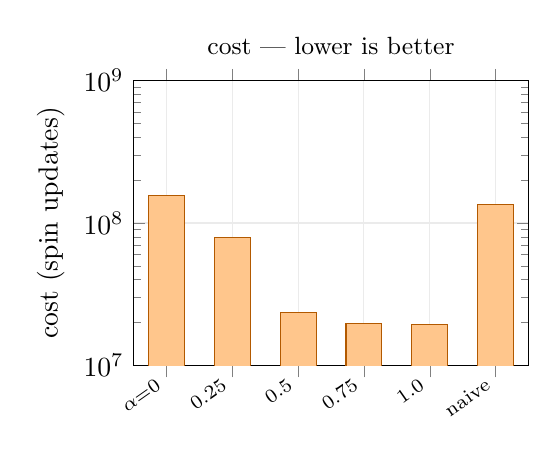
\begin{tikzpicture}
\begin{axis}[width=6.6cm,height=5.2cm,ybar,bar width=13pt,ymode=log,
 symbolic x coords={$\alpha$=0,0.25,0.5,0.75,1.0,naive},xtick=data,
 x tick label style={font=\scriptsize,rotate=35,anchor=east},
 ylabel={cost (spin updates)},ymin=1e7,ymax=1e9,
 title={\small cost --- lower is better},grid=major,grid style={gray!16}]
\addplot[fill=orange!45,draw=orange!70!black] coordinates
 {($\alpha$=0,1.55e8) (0.25,7.89e7) (0.5,2.35e7) (0.75,1.98e7) (1.0,1.94e7) (naive,1.34e8)};
\end{axis}
\end{tikzpicture}
\caption{\MEAS{} EA spin glass, $L=16$, $R=30$, 6 thresholds, full $6/6$ coverage at every
allocation. Left: uniform allocation ($\alpha=0$) is the \emph{flattest}; every FW-CADIS setting
is worse, and not even monotonic in $\alpha$. Right: FW-CADIS runs at $\sim8\times$ lower cost.
The cost advantage is real; the flattening advantage is not present.}
\label{fig:fwcadis}
\end{figure}

At the most favourable configuration tested ($R=90$, shallowest threshold family), uniform gives
flatness $276.1$ with CI $[224,344]$ against FW-CADIS $297.3$ with CI $[234,388]$; the
paired-difference estimate is $+20.9$ with CI $[-77.2,+137.6]$, including zero. Confidence-interval
width scaled as $1/\sqrt{R}$ (predicted shrink $0.577$, observed $0.597$); resolving the remaining
gap would need $R\approx2300$, and given the consistent direction such a run would most likely
confirm \emph{uniform} as flatter. It was not run.

%==========================================================
\section{Implementation Notes}
%==========================================================

\subsection{Vectorisation: the dominant avoidable cost}
NumPy overhead is paid per call, so throughput depends strongly on population size:

\begin{table}[H]\centering\small
\caption{\MEAS{} \texttt{sweep\_population} throughput, $L=16$.}
\begin{tabular}{cccc}\toprule
population & ms/sweep & $\mu$s per walker-sweep & overhead\\\midrule
1 & 0.184 & 184.2 & $8.6\times$\\
10 & 0.304 & 30.4 & $1.4\times$\\
100 & 2.299 & 23.0 & $1.1\times$\\
1000 & 21.372 & 21.4 & $1.0\times$\\
2500 & 59.984 & 24.0 & $1.1\times$\\
\bottomrule\end{tabular}
\end{table}

Label generation originally looped over configurations one at a time, issuing
$2500\times400=10^6$ calls at population 1 --- the worst point on the curve. Rollouts are
independent across configurations, so the loop batches exactly:

\begin{lstlisting}[language=Python,caption={Batched label generation: measured 8.6$\times$ faster, statistically identical output.}]
def generate_milestone_labels(S, T, Jx, Jy, model, milestones, n_roll, roll_K, rng):
    bulk, target = float(milestones[0]), float(milestones[-1])
    S = S.copy()
    best = energy_per_spin(S, Jx, Jy)          # shape (n,), not (1,)
    for _ in range(n_roll):
        for _ in range(roll_K):
            S = sweep_population(S, T, Jx, Jy, rng)
        best = np.minimum(best, energy_per_spin(S, Jx, Jy))
    return np.clip((best - bulk) / (target - bulk), 0.0, 1.0)
\end{lstlisting}

Verified at $n=300$: looped $21.4$\,s, batched $2.48$\,s; label mean $0.4743$ vs $0.4779$,
identical maximum. RNG consumption order differs, so cached labels from the looped version must
be discarded when switching.

\subsection{On GPU acceleration}
Not currently justified. Network training is $\approx1\%$ of wall time. The Monte Carlo dominates
but working arrays are $\sim1$\,MB, and a checkerboard sweep is two kernel launches over
$\sim10^5$ trivial operations --- launch latency is comparable to the work. Replica-level
parallelism across CPU cores is already near-linear. GPU becomes attractive at $L\ge64$ with
populations of $10^4$, at which point the change is porting \texttt{sweep\_population} to tensors,
not the network.

\subsection{Figure of merit and its degenerate cases}
\begin{equation}
\mathrm{FOM}=\frac{1}{\sigma^2_{\mathrm{rel}}\cdot\text{cost}},\qquad
\sigma^2_{\mathrm{rel}}=\frac{\mathrm{Var}[\hat\pi]}{\mathbb{E}[\hat\pi]^2}\ (\text{ddof}=1).
\end{equation}
FOM is meaningful only as a \emph{ratio between methods on the same problem with the same cost
metric}; its absolute magnitude carries the units of cost and no universal threshold applies.
Report $\mathrm{FOM}=0$ when the event was never observed and $\mathrm{NaN}$ when fewer than two
replicas prevent a variance estimate --- never $\infty$.

\begin{warnbox}{Statistical floor on replica count}
With few replicas and frequent zeros, the reported relative standard deviation is an algebraic
artefact, not a measurement. For replica vectors $[x,0,0,0]$ it is exactly $2.000$; for
$[a,a,0,0]$ exactly $2/\sqrt3=1.1547$. Both patterns appeared in early runs. \textbf{Do not
interpret rel.\,sd when the zero count is comparable to the replica count.} Use $R\ge20$ and
report the zero count beside every FOM.
\end{warnbox}

%==========================================================
\section{Pipeline and Reproduction}
%==========================================================

\begin{figure}[H]\centering
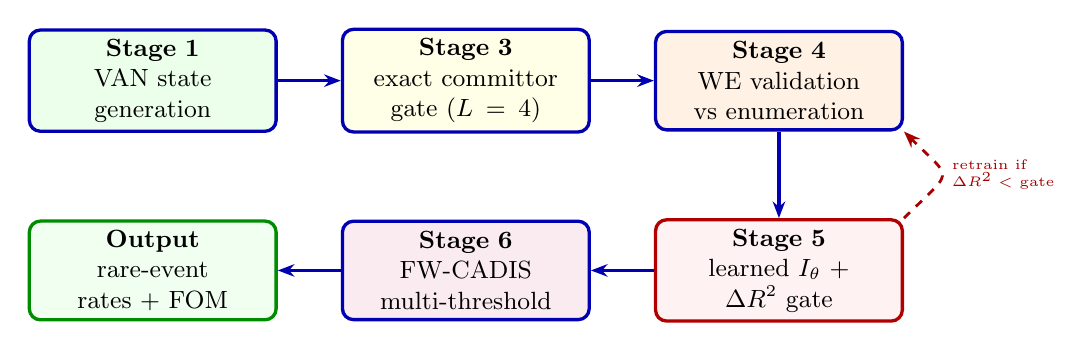
\begin{tikzpicture}[node distance=1.0cm and 0.7cm,
 stage/.style={rectangle,draw=blue!70!black,fill=blue!5,very thick,text width=2.9cm,
   text centered,rounded corners,minimum height=1.25cm,font=\small},
 audit/.style={rectangle,draw=red!70!black,fill=red!5,very thick,text width=2.9cm,
   text centered,rounded corners,minimum height=1.25cm,font=\small},
 outnode/.style={rectangle,draw=green!55!black,fill=green!6,very thick,text width=2.9cm,
   text centered,rounded corners,minimum height=1.25cm,font=\small},
 ar/.style={draw,-{Stealth[length=6pt]},line width=1.2pt,blue!70!black}]
\node [stage,fill=green!8] (s1) {\textbf{Stage 1}\\VAN state generation};
\node [stage,right=0.8cm of s1,fill=yellow!10] (s3) {\textbf{Stage 3}\\exact committor gate ($L=4$)};
\node [stage,right=0.8cm of s3,fill=orange!10] (s4) {\textbf{Stage 4}\\WE validation vs enumeration};
\node [audit,below=1.1cm of s4] (s5) {\textbf{Stage 5}\\learned $I_\theta$ $+$ $\Delta R^2$ gate};
\node [stage,left=0.8cm of s5,fill=purple!8] (s6) {\textbf{Stage 6}\\FW-CADIS multi-threshold};
\node [outnode,left=0.8cm of s6] (o) {\textbf{Output}\\rare-event rates $+$ FOM};
\path [ar] (s1)--(s3); \path [ar] (s3)--(s4); \path [ar] (s4)--(s5);
\path [ar] (s5)--(s6); \path [ar] (s6)--(o);
\path [draw,-{Stealth[length=6pt]},dashed,line width=1pt,red!65!black]
 (s5.north east) .. controls +(45:0.9cm) and +(-45:0.9cm) .. (s4.south east)
 node[pos=0.5,right,font=\tiny,align=left]{retrain if\\$\Delta R^2<$ gate};
\end{tikzpicture}
\caption{\SCHEM{} Execution graph. Every stage is gated against an exact or enumerable reference
before the next is trusted; the dashed edge is the diagnostic feedback loop.}
\label{fig:pipeline}
\end{figure}

\subsection{Reproduction commands}
\begin{lstlisting}[language=bash,caption={Reference invocations. Delete the label cache whenever the labelling function changes.}]
python3 run_all.py --preset laptop            # full pipeline, ~1 h
python3 run_all.py --preset smoke             # fast correctness check
python3 run_all.py --preset laptop --only 4 5 # weight windows + learned coordinate

rm -rf .label_cache/
python3 05_neural_importance/run_milestone.py --model ea --preset custom \
        --beyond 1 --replicas 20 --jobs 7 --tau 2
\end{lstlisting}

%==========================================================
\section{Bug Log}
%==========================================================

Six implementation faults are recorded. Three produced plausible-looking, internally consistent
wrong numbers caught only by independent diagnostics; one was caught before it could affect any
number. This is included as a section rather than a footnote because the diagnostic reasoning is
the reusable part.

\begin{table}[H]\centering\small
\caption{Bugs found, in order of discovery.}
\begin{tabular}{p{2.5cm}p{11.6cm}}\toprule
\textbf{Where} & \textbf{What, and how it surfaced}\\\midrule
Weight-window ladder &
Bin-range upper edge calibrated against random, infinite-temperature configuration energy
($\approx0$) instead of equilibrium ($\approx-0.72$), wasting over half the bin resolution.
Surfaced by the contradiction between poor WE scores and the incremental-$R^2$ diagnostic's
claim that $I_\theta$ carried real information. Confirmed by a before/after rerun in which
\emph{only} the exposed method moved, by the predicted amount, and everything else was
bit-identical.\\\midrule
Self-consistency degeneracy &
The self-consistency equation plus a single (target) boundary condition is under-determined:
$I\equiv1$ satisfies it exactly for any amount of data, so training collapses to a useless flat
coordinate while reporting a small loss. Surfaced by instrumenting the trained output's spread
($\mathrm{sd}<0.01$), \emph{not} by the loss curve, which looked normal. Fixed with a second
boundary condition anchoring bulk states to a distinct reference value.\\\midrule
Resampling interval &
Hard-coded at 20 sweeps, roughly $20\times$ the system's own $\approx1$-sweep correlation time
(Fig.~\ref{fig:relax}), letting split walkers fully relax before the next resampling and silently
degenerating every WE variant to naive-with-overhead. Surfaced by every WE variant scoring worse
than plain naive, contrary to all other results.\\\midrule
Collection depth &
The self-consistency training pass used iteration and walker budgets tuned for the surrogate
objective, far shallower than the evaluation depth, so it never collected a state within one
spin-flip of the target and the target boundary condition could not fire. Surfaced by an explicit
warning from the training code; confirmed structural by reproducing at two lattice sizes and two
depths before fixing (44 boundary states found versus 0).\\\midrule
Inverted milestone labels
\textcolor{green!45!black}{(no number affected)} &
\texttt{searchsorted} on ascending-sorted milestones placed the target at index 0, training the
network as an anti-importance function. Surfaced by tracing why label statistics moved the wrong
way when the target was deepened. WE binning is orientation-agnostic (affine flip preserves the
bin partition), so no reported result changed --- but the same coordinate used for Doob tilting
or source biasing would have driven walkers \emph{away} from the target.\\\midrule
Unseeded network initialization\label{man:seedbug}
\textcolor{red!55!black}{(headline number affected)} &
\texttt{run\_milestone.py} never called \texttt{torch.manual\_seed}, so the trained network's
random weight initialization varied silently between runs of an otherwise byte-identical
configuration (same cached labels, hyperparameters, $\tau=2$). Surfaced while attempting to
bootstrap the milestoning headline for publication: a second run of the identical config gave
WE[$I_\theta$] a $17\%$ \emph{loss} against WE[$E$], reversing the original run's $14\%$ win.
Fixed with an explicit seed plus a \texttt{--net-seed} sweep flag; the fix itself was confirmed
complete by running seed 0 twice and reproducing bit-for-bit (including full wall-clock
trajectory). Unlike the other faults here, this one had already produced a reported result that
looked validated (bootstrapped, $0/10$ zero-replicas) before the second run exposed it --- the
single most consequential catch in this project, since the original number would otherwise have
shipped as a clean win. See \S\ref{sec:milestoneresults} for the full seed sweep.\\
\bottomrule\end{tabular}
\end{table}

Additional faults affecting robustness rather than reported numbers --- silent single-core
fallback when a coordinate object failed to pickle across worker processes, a degenerate FOM case
returning $\infty$ instead of NaN, a threshold calibrator that clamped and printed a false rarity
claim on small lattices --- were found in a logic audit and are not repeated here.

%==========================================================
\section{Verification Status}\label{sec:status}
%==========================================================

Claims are graded: \textbf{[E]} exact (theorem-level, or matching an exact reference to numerical
precision); \textbf{[V]} validated (bootstrap CI or equivalent statistical control);
\textbf{[O]} open (point estimate or unresolved).

\begin{table}[H]\centering\small
\begin{tabular}{p{7.6cm}cp{5.2cm}}\toprule
\textbf{Claim} & \textbf{Grade} & \textbf{Basis}\\\midrule
Adjoint importance $\equiv$ committor & [E] & Theorem~\ref{thm:zv}\\
Exact-committor tilt is zero-variance & [E] & measured rel.\ var.\ $\sim10^{-30}$\\
Approximate tilt without weight windows is worse than naive & [E] & 1D toy walk\\
WE unbiased for any coordinate & [E] & weight-conservation identity\\
WE matches exact enumeration at $L=4$ & [E] & $|\Delta\ln P|=0.006$--$0.024$\\
WE reaches $\sim$2 decades deeper than naive at matched cost & [V] & $L=20$ tail\\
$\tau_{\mathrm{corr}}\approx1$ sweep at $T=2.6$ & [E] & Fig.~\ref{fig:relax}\\
$\tau=20$ destroys the WE ratchet & [E] & front-penetration table\\
$\tau=4$ ``restores'' control & \textbf{withdrawn} & fails to reach target bin at depth\\
Fixed bin ladder cheaper than adaptive & [V] & 40\% cost reduction\\
Bin \emph{width} controls reach & \textbf{withdrawn} & controlled test: identical hit rate\\
$I_\theta$ carries information beyond $E$ & [V] & $\Delta R^2=+0.250$ vs noise floor $0.02$\\
Milestoning beats WE[$E$] & [O] & 17-seed two-level bootstrap CI $[0.84,1.75]$, includes 1\\
Batched labelling $8.6\times$ faster & [E] & timing at $n=300$\\
Frustration $49.2\%$ at seed 0 & [E] & plaquette count\\
Self-consistency beats surrogate objective & [O] & CI includes 1; effect shrinks with $R$\\
FW-CADIS flattens relative error & \textbf{negative} & uniform flatter at every $\alpha$\\
FW-CADIS $\sim8\times$ cheaper & [V] & Fig.~\ref{fig:fwcadis}\\
Any learned coordinate beats \emph{naive} outright & [O] & naive leads raw FOM in every clean run\\
\bottomrule\end{tabular}
\end{table}

\subsection{What remains open}
Whether milestoning genuinely beats WE[$E$] at all is unresolved after seventeen seeds: the point
estimate is stably positive but modest ($\sim\!1.2\times$) across four independent bootstrap
checkpoints, and the CI cannot be closed by seed count alone at a cost proportionate to the
question ($\sim\!100$ seeds, $\sim$40h, to exclude 1). Whether any learned coordinate beats plain
naive Monte Carlo outright --- rather than merely the best hand-picked coordinate --- is likewise
unresolved: naive retains the best raw FOM in every clean comparison so far, regardless of seed.
Whether FW-CADIS's failure to flatten is a property of this energy landscape, of the
bin/threshold parameterisation, or a general limit at this scale would need a different problem
instance, not more replicas of this one. Push-to-scale questions --- three dimensions, larger $L$
--- are untouched (\S\ref{sec:threed} states precisely what would change and what would not).

\begin{thebibliography}{99}
\bibitem{wu2019} D. Wu, L. Wang, P. Zhang, \emph{Solving Statistical Mechanics Using Variational
Autoregressive Networks}, Phys. Rev. Lett. \textbf{122}, 080602 (2019); arXiv:1809.10606.
\bibitem{wagner1998} J. C. Wagner, A. Haghighat, \emph{Automated Variance Reduction of Monte
Carlo Shielding Calculations Using the Discrete Ordinates Adjoint Function (CADIS)},
Nucl. Sci. Eng. \textbf{128}, 186 (1998).
\bibitem{wagner2014} J. C. Wagner, D. E. Peplow, S. W. Mosher, \emph{FW-CADIS Method for Global
and Regional Variance Reduction of Monte Carlo Radiation Transport Calculations},
Nucl. Sci. Eng. \textbf{176}, 37 (2014).
\bibitem{cooper2001} M. A. Cooper, E. W. Larsen, \emph{Automated Weight Windows for Global Monte
Carlo Particle Transport}, Nucl. Sci. Eng. \textbf{137}, 1 (2001).
\bibitem{zuckerman2017} D. M. Zuckerman, L. T. Chong, \emph{Weighted Ensemble Simulation: Review
of Methodology, Applications, and Software}, Annu. Rev. Biophys. \textbf{46}, 43 (2017).
\bibitem{ev2006} W. E, E. Vanden-Eijnden, \emph{Towards a Theory of Transition Paths},
J. Stat. Phys. \textbf{123}, 503 (2006).
\bibitem{doobvan} \emph{Nonequilibrium Statistical Mechanics Revealed by Doob Transform and
Variational Autoregressive Networks}, Phys. Rev. E \textbf{111}, 034120 (2025).
\bibitem{spanier} J. Spanier, E. M. Gelbard, \emph{Monte Carlo Principles and Neutron Transport
Problems} (1969).
\bibitem{kim} M. Kim, W. Cai, \emph{Accelerated MCMC via neural network-driven importance
sampling} (2026). \textbf{[arXiv identifier requires verification before submission.]}
\bibitem{onsager1944} L. Onsager, \emph{Crystal statistics. I. A two-dimensional model with an
order-disorder transition}, Phys. Rev. \textbf{65}, 117 (1944).
\bibitem{talapov1996} A. L. Talapov, H. W. J. Bl\"ote, \emph{The magnetization of the 3D Ising
model}, J. Phys. A \textbf{29}, 5727 (1996).
\bibitem{binderyoung1986} K. Binder, A. P. Young, \emph{Spin glasses: Experimental facts,
theoretical concepts, and open questions}, Rev. Mod. Phys. \textbf{58}, 801 (1986).
\bibitem{hasenbusch2008} M. Hasenbusch, A. Pelissetto, E. Vicari, \emph{Critical behavior of
three-dimensional Ising spin glass models}, Phys. Rev. B \textbf{78}, 214205 (2008).
\bibitem{adzhemyan2022} L. Ts. Adzhemyan, D. A. Evdokimov, M. Hnati\v{c}, E. V. Ivanova,
M. V. Kompaniets, A. Kudlis, D. V. Zakharov, \emph{The dynamic critical exponent $z$ for 2d and
3d Ising models from five-loop $\varepsilon$ expansion}, Phys. Lett. A \textbf{425}, 127870
(2022).
\end{thebibliography}

\end{document}
